% GRASP: Copyright 1997,1998,1999  Bruce Allen
% $Id: man_utility.tex,v 1.38 1999/07/11 21:22:18 ballen Exp $
\section{GRASP Routines: General purpose utilities}
\label{s:utility}
\setcounter{equation}0
This section includes general purpose utility functions for a variety
of purposes.  For example, these include functions for error handling,
to calculate time-averaged power spectra, and functions to graph data,
listen to data, etc.
\clearpage
\subsection{GRASP Error Handling}
\setcounter{equation}0
\label{ss:errors}

GR\_error is the GRASP error reporting module.  It has two abstract
interfaces which insulate the GRASP library and the programs which use
it from the details of how GRASP will report errors and how the program
will handle them.  The internal interface provides GRASP itself with a
standard method to report errors.  The external interface allows
programs which use GRASP to specify exactly how error reports are to be
handled.  In addition, a default set of handling routines is provided
for printing error messages in a standard format to stderr or a log
file.

If you are writing a package for GRASP, here is an example of how to
call the error handler.  The following sections contain more detailed
information, but this example is a userful summary of ``how to use
it''. Please note that you {\it must} include ``newline" characters
${\tt \backslash n}$ in your {\tt GR\_report\_error()} calls.  If you fail to do
this the lines of error messages will all be strung together on a single line!
{\tt 
\begin{verbatim}
...
/* first call GR_start_error() to begin the error message */
GR_start_error("trouble()",rcsid,__FILE__,__LINE__);
/* then call GR_report_error() as many times as desired */
GR_report_error("The GR_report_error() function is like printf().\n");
GR_report_error("It can have no arguments.\n");
GR_report_error("It can have a float argument %f\n",x1);
GR_report_error("Or any mixture of valid types %d %d %%s\n",i1,i2,stringptr);
/* finally, call GR_end_error() to terminate the error message */
GR_end_error();
...
\end{verbatim}}
\noindent
The use of these three routines as shown will print out, for example:
{\tt 
\begin{verbatim}
GRASP: Message from function trouble() at line number 123 of file "source.c".
The GR_report_error() function is like printf().
It can have no arguments.
It can have a float argument 5.43210
Or any mixture of valid types -2 17 the string pointed to by the pointer
$Id: man_utility.tex,v 1.38 1999/07/11 21:22:18 ballen Exp $
$Name: RELEASE_1_9_8 $
\end{verbatim}}
\noindent
In particular, the line number, release number, and file name are all
filled in automatically. 

\subsubsection{Reporting Errors In GRASP Code}

Reporting errors from within GRASP code is simple: every legal GRASP
error report consists of exactly one call to {\tt GR\_start\_error()},
zero or more calls to {\tt GR\_report\_error()}, and exactly one call
to {\tt GR\_end\_error()}.  Failing to call the functions in exactly
this order will cause an assert to fail and the program to abort; this
allows the code in the handler routines to safely assume that they will
be called in the correct order.

{\tt GR\_start\_error()} takes four arguments specifying the name of
the function in which the error occured, the RCS ID of the GRASP file
which contains the function's source, the name of that file, and the
line number on which the error report began.  In practice providing
this data is easy.  Every GRASP file should declare a static string
'rcsid' containing the ID, and ANSI C defines the macros \_\_FILE\_\_
and \_\_LINE\_\_ which expand to the file name and line number,
respectively.  Within a given file only the function name parameter
will change from call to call.

The arguments to {\tt GR\_report\_error()} are exactly the same as
those to printf(): a familiar printf-style format string followed by a
variable number of arguments.  There is no file pointer a' la fprintf()
because the errors may not be printed to a file or the screen but
handled in some completely different way determined by the calling
program.  Repeated calls are a convenient way to build up the complete
message just as with printing to the screen with printf().  Finally, a
call to {\tt GR\_end\_error()} ends the report.  It requires no
arguments.

The GRASP source code provides many examples of the use of these
functions, and they are documented by example in
Section~\ref{ss:errors}.  Because of the stereotyped calling sequence
and arguments involved, an efficient technique for GRASP library
programmers is to paste in the calls from another location in the
source file or from a handy template kept in a scratch file so that
only the function name and actual message needs editing for each case.


\subsubsection{How GRASP Error Reports Are Handled}
Programs vary widely in how they notify the user of errors.  A simple
command-line program will probably print the messages to the screen or
a file, while a program with a graphical interface will likely send
them to an error log window or to a dialog window.  GRASP allows
arbitrary error handlers to be specified, but the default provided will
probably suffice for most GRASP application programmers.

Calling GR\_set\_errors\_enabled() with an argument of false (zero)
will suppress all GRASP error messages regardless of the actual
handlers used, while a true argument will enable them again.
GR\_errors\_enabled() returns true if errors are currently enabled and
false otherwise.  Errors always start out enabled unless the
environment variable 'GRASP\_NODEBUG' exists (its value is irrelevant),
in which case they are disabled by default.  Errors may be disabled
within a handler, but the change will not take place until the next
{\tt GR\_start\_error()} call.

By default, the default error handlers print errors to stderr.  The
function, file, and line number are reported in a standard header
format, followed by the message itself printed as though each call to
GR\_report\_error(format, args) was a call to fprintf(stderr, format,
args), and ending with the RCS ID of the file containing the function
source.  If the environment variable 'GRASP\_ERRORFILE' exists and its
value is the pathname of a file which can be opened for appending that
filename is used instead of stderr.  Finally, if in addition
'GRASP\_ERRORFILE\_OVERWRITE' exists (its value is irrelevant) the file
is overwritten rather than appended to.

\subsubsection{Customizing The Default Handlers}

GRASP error reports may be customized by modifying the behavior of the
default handler functions or by replacing them entirely.  By default,
when {\tt GR\_start\_error()} is called it checks to see if there is a
default file name set; if so, that file is opened for appending.  If
not (that is, if the filename has been set to NULL), or if the file
cannot be opened, it then checks to see if an error FILE* has been
set.  If so, that file is used.  If not, then the handler fails since
it has no way to report the error.  The default {\tt
GR\_report\_error()} prints to whatever file {\tt GR\_start\_error()}
chose to use, and {\tt GR\_end\_error()} prints the RCS ID.  If the
file was opened by name in {\tt GR\_start\_error()} then {\tt
GR\_end\_error()} also closes it.

The default FILE* can be set and examined with GR\_set\_error\_file()
and GR\_get\_error\_file(), and the default filename can be set and
examined with GR\_set\_error\_file\_name() and
GR\_get\_error\_file\_name().  The default behavior can be restored
with GR\_set\_error\_file(stderr) and/or
GR\_set\_error\_file\_name(NULL).  These functions may be called at any
time except during an error report (between the calls to {\tt
GR\_start\_error()} and {\tt GR\_end\_error()}), when an assert would
fail.  (This is a non-issue in practice because the file/filename could
only be changed during a report if the file or filename is set in GRASP
code itself, if the error reporting functions are called in user code
as well as in GRASP, or if a custom handler changes the file/filename
and then calls the default handler.  The first possibility is strictly
forbidden, and the others are discouraged because they can lead to
confusion and subtle bugs.)

The reason for this somewhat complex system is safety.  If a specified
file name cannot be opened errors can still be reported to the FILE*,
probably stderr.  If an error file name has been set, the file is
opened and closed for each report so that if the program crashes as
much of the error log as possible is preserved on disk.

When using GR\_set\_error\_file(), the calling program is responsible
for opening the file for writing before the call and closing it (if
necessary); GRASP will simply assume that the file is always available
for output.  A NULL file pointer is allowed, in which case calls to the
default error handler will cause an assert to fail unless an error file
name has been set.

When a file name is set with GR\_set\_error\_file\_name(), GRASP
immediately attempts to open the file.  If the erasefile parameter is
TRUE (nonzero) the file will be opened for writing, if it is false
(zero) it will be opened for appending.  If the open succeeds, the name
is copied and stored for future use (this means that the function can
be safely called with locally allocated storage), an identifying
start-up message and the time is written to the log file (even if error
reporting is disabled), the file is closed, and the function returns
true.  When appending to a non-empty file it also writes a separator
line so that reports from different runs are more easily
distinguished.  If the open fails, the filename is left unchanged (if a
previous one existed), an error is reported in the usual way (unless
error messages are suppressed), and the function returns false.
Setting a NULL filename means that the FILE* should be used instead;
the erasefile parameter is ignored in this case and the call always
succeeds.  As with GR\_set\_error\_file(), the filename may not be
changed during a report.

It is easy to see how the default behavior is obtained using these
handlers.  The default FILE* is stderr; conceptually a call to
GR\_set\_error\_file(stderr) occurs before the program begins.
Similarly, a conceptual call to GR\_set\_error\_file\_name(filename,
erase) occurs before program execution, with filename having the value
of the environment variable GRASP\_ERRORFILE if it exists and NULL
otherwise, and erase true if the environment variable
GRASP\_ERRORFILE\_OVERWRITE exists and false otherwise.

\subsubsection{Writing Custom Error Handlers}

Internally, GR\_error keeps three pointers of type
GR\_start\_error\_type, GR\_report\_error\_type, and
GR\_end\_error\_type (defined in grasp.h) which point to the current
start\_error, report\_error, and end\_error handlers, respectively.
When the three error handlers {\tt GR\_start\_error()}, {\tt
GR\_report\_error()}, and {\tt GR\_end\_error()} are called, they in
turn check to see that they are called in the proper order and then
call the function pointed to by the corresponding function pointer if
(and only if) the function pointer is non-NULL (so that for convenience
if a particular handler is not neccessary a dummy routine is not
required) and if errors are currently enabled (so disabling errors
works regardless of the handler).  By default the handler pointers
simply reference GR\_default\_start\_error(),
GR\_default\_report\_error(), and GR\_default\_end\_error(), which
actually implement the default behavior described above.  For
convenience they may be restored with GR\_restore\_default\_handlers()
as well as GR\_set\_error\_handlers().

The functions GR\_set\_error\_handlers() and GR\_get\_error\_handlers()
set and examine the handler's current values, so that by writing the
proper functions GRASP's error reports can be customized in any way
desired.  The GR\_...\_error\_type typedef's in grasp.h illustrate the
proper function prototypes.  Note that GR\_report\_error\_type
functions take a va\_list as their second argument rather than '...';
for convenience {\tt GR\_report\_error()} creates the list and calls
va\_start() beforehand and calls va\_end() afterwards so the handler
need only deal with the list itself.  In the common case where the
message will simply be printed to a file, the va\_list may be passed
directly to one of the v...printf functions.  The only restriction is
that the handlers may not be changed between calls to {\tt
GR\_start\_error()} and {\tt GR\_end\_error()}, but just as when
changing the default error files this should not be a problem in
practice.

The default handlers in {\tt src/utility/GR\_error.c} and their
supporting routines are good examples of how GRASP error handlers are
written.  They are special only in that they are initialized and set
automatically; otherwise, they use only features available to any
handler.  Most of their code provides the ability to switch files
easily and safely; writing a custom handler that does not need this
generality is quite straightforward.  GR\_is\_reporting() returns true
if a report is in progress and is sometimes useful when writing custom
handlers.

\clearpage
\subsubsection{Functions: {\tt GR\_start\_error()}, {\tt GR\_report\_error()}, {\tt GR\_end\_error()}}
\label{ss:error}

These three functions are the GRASP error handlers.  Their use is best
illustrated by example.  A typical usage is shown below -- a fragment
taken from a fictitous routine called ``{\tt trouble()}".
{\tt 
\begin{verbatim}
...
GR_start_error("trouble()",rcsid,__FILE__,__LINE__);
GR_report_error("The GR_report_error() function is like printf().\n");
GR_report_error("It can have no arguments.\n");
GR_report_error("It can have a float argument %f\n",x1);
GR_report_error("Or any mixture of valid types %d %d %s\n",i1,i2,stringptr);
GR_end_error();
...
\end{verbatim}}
\noindent
The use of these three routines as shown will print out, for example:
{\tt 
\begin{verbatim}
GRASP: Message from function trouble() at line number 123 of file "source.c".
The GR_report_error() function is like printf().
It can have no arguments.
It can have a float argument 5.43210
Or any mixture of valid types -2 17 the string pointed to by the pointer
$Id: man_utility.tex,v 1.38 1999/07/11 21:22:18 ballen Exp $
$Name: RELEASE_1_9_8 $
\end{verbatim}}
\noindent
In particular, the line number, release number, and file name are all
filled in automatically.  The environment variables that govern the
behavior of the default error handler are shown in
Table~\ref{t:errorenv} below.
\begin{table}[b]
\begin{tabular}{lp{3 in}}
Environment variable. & How to set, and effect obtained.\\
\hline 
{\tt GRASP\_NODEBUG}  & {\tt setenv GRASP\_NODEBUG}  $\qquad \qquad \qquad $ turns off error messages. \\
{\tt GRASP\_ERRORFILE}  &  {\tt setenv  GRASP\_ERRORFILE thisfile} sends errors to file ``{\tt thisfile}". \\
{\tt GRASP\_ERRORFILE\_OVERWRITE}  &  {\tt setenv  GRASP\_ERRORFILE\_OVERWRITE} errors don't accumulate in file.
\end{tabular}
\caption{The behavior of the error handler is determined by three
environment variables, which can be set and un-set using the shell
commands {\tt setenv} and {\tt unsetenv}.  These permit the error
messages to be turned off, saved in a file, and control the file name
and its over-write properties.}
\label{t:errorenv}
\end{table}

\clearpage
\subsection{Function: {\tt grasp\_open()}}
\label{ss:graspopen}
\setcounter{equation}0
{\tt 
FILE* grasp\_open(const char *environment\_variable,const char *shortpath,const char *mode) }

This routine provides a simple mechanism for obtaining the pointer to a
data or parameter file.  It is called with two character strings.
One of these is the name of an environment variable, for example
{\tt GRASP\_DATAPATH} or {\tt GRASP\_PARAMETERS}.  The second argument
is the ``tail end" of a path name.  The routine then constructs a path
name whose leading component is determined by the environment variable
and whose tail end is determined by the short path name.  {\tt grasp\_open()}
opens the file (printing useful error messages if this is problematic) and
returns a pointer to the file.  

The arguments are:
\begin{description}
\item{\tt environment\_variable:} Input.  Pointer to a character string
   containing the name of the environment variable.
\item{\tt shortpath:} Input.  Pointer to a character string containing
   the remainder of the path to the file.
\item{\tt mode:} Input.  File mode. Pointer to a character string containing
   "r" if you want to read the file, "w" if you want to write to the
   file, and so on.  A list of the possible modes is:
\begin{verbatim}
     r or rb            open file for reading
     w or wb            truncate to zero length or create file for
                        writing
     a or ab            append; open or create file for writing at
                        end-of-file
     r+ or rb+ or r+b   open file for update (reading and writing)
     w+ or wb+ or w+b   truncate to zero length or create file for
                        update
     a+ or ab+ or a+b   append; open or create file for update,
                        writing at end-of-file
\end{verbatim}
\end{description}

As a simple example, if the environment variable {\tt GRASP\_PARAMETERS}
is set to\\
{\tt /usr/local/data/14nov94.2}\\
and one calls\\
{\tt grasp\_open("GRASP\_PARAMETERS","channel.0","r")}\\
then the routine opens the file\\
\mbox{\tt /usr/local/data/14nov94.2/channel.0}\\
for reading and returns a pointer to it.
\clearpage

\subsection{Function: {\tt avg\_spec() }}
\setcounter{equation}0
{\tt 
void avg\_spec(float *data,float *average,int npoint,int *reset,float srate,float decaytime,int windowtype,int overlap)}

This routine calculates the power spectrum of the (time-domain) input
stream {\tt data[ ]}, averaged over time with a user-set exponential
decay, several possible choices of windowing and the possibility to
overlap data in subsequent calls.

The arguments are:
\begin{description}
\item{\tt data:} Input.  The time domain input samples are contained in
{\tt data[0..N-1]}, with the data sample at time $t= n \Delta t$
contained in {\tt data[n]}.
\item{\tt average:} Output.  The one sided power spectrum is returned in
{\tt average[0,..N/2-1]}.  The value of {\tt average[m]} is the
average power spectrum at frequency
\begin{equation}
f={{\tt m} \times {\tt srate} \over {\tt N}}.
\end{equation}
We do not output the value of the average at the Nyquist frequency,
which would be the (non-existent) array element {\tt average[N]}.  The
units of {\tt average[ ]} are ${\tt data[ ]}^2/{\rm Hz}$.  Note: the
elements of {\tt average[ ]} must not be changed in between successive
calls to {\tt avg\_spec()}.
\item{\tt npoint:} Input.  The number of points ${\tt npoint}=N$
input.  This must be an integer power of two.
\item{\tt reset:} Input.  If set to zero, then any past contribution to
the average power spectrum is initialized to zero, and a new average is
begun with the current input data.
\item{\tt srate:} Input.  The sample rate $1/\Delta t$ of the input
data, in Hz.
\item{\tt decaytime:} Input.  The characteristic (positive) decay time
 $\tau$ in seconds, to use for the moving (exponentially-decaying)
 average described below.  If no averaging over time is wanted, simply
 set {\tt decaytime} to be small compared to $N \Delta t$.
\item{\tt windowtype:} Input.  Sets the type of window used in power
spectrum estimation.  Rectangular windowing (i.e., no windowing) is
{\tt windowtype=0}, Hann windowing is  {\tt windowtype=1}, Welch
windowing is {\tt windowtype=2} and Bartlett windowing is {\tt
windowtype=3}.  See \cite{NumRec} for a discussion of windowing and the
definitions of these window types.
\item{\tt overlap:} Input.  Must be either zero or unity.  If set to
unity, then the data is overlapped by $N/2$ points with previous data
(see below for a description of the overlapping procedure).   When set
to zero no overlapping is performed.
\end{description}

The methods used in this routine are quite similar to those used in
the {\it Numerical Recipes} \cite{NumRec} routine {\tt spctrm()}, and
the reader interested in the details of this routine should first read
the corresponding section of \cite{NumRec}.  Note that to reproduce
(exactly) the procedure described in {\it Numerical Recipes}
\cite{NumRec} one must have {\tt npoint}=2$\times$M where M is the
variable used in the procedure {\tt spctrm()}, and the decay time must
be very large (so that the two successive spectra are equally
weighted).  If the data being passed is not continuous from one call
to the next, set {\texttt overlap}=0.

One frequently  wants to do a moving-time average of power spectra, for
example to see how the noise spectral properties of an interferometer
are changing with time.  This is accomplished in {\tt avg\_spec()} by
averaging the spectrum with an exponentially-decaying average.  Let
$A_{t}(f)$ denote the average power spectrum as a function of frequency
$f$, at time $t$.  Then the exponentially-decaying average ${\langle
A(f) \rangle}_t$ at time $t$ is defined by
\begin{equation}
\label{e:defavg}
{\langle A(f) \rangle}_t = {
  \int_{-\infty}^t dt' \;  A_{t'}(f) {\rm e}^{-(t-t')/\tau} 
\over 
  \int_{-\infty}^t dt' \; {\rm e}^{-(t-t')/\tau} 
},
\end{equation}
where $\tau$ is the characteristic decay time over which an impulse in
the power spectrum would decay.  In our case, we wish to average the
power spectra obtained in the nth pass through the averaging routine.
The discrete analog of the previous equation (\ref{e:defavg}) is
\begin{equation}
\label{e:defavg2}
{\langle A(f) \rangle}_N = {
  \displaystyle \sum_{n=0}^N  A_n(f) {\rm e}^{-\alpha (N-n) } 
\over 
\displaystyle  \sum_{n=0}^N {\rm e}^{-\alpha (N-n) } 
}.
\end{equation}
Here, 
\begin{equation}
\alpha = { {\tt npoint} \over {\tt srate} \times {\tt decaytime} }
\end{equation}
is determined by the averaging time desired.  The average defined by
(\ref{e:defavg2}) can be easily determined by a recursion relation.  We
denote the the normalization factor by
\begin{equation}
{\cal N}_N = \sum_{n=0}^N {\rm e}^{-\alpha (N-n) }.
\end{equation}
It obeys the (stable) recursion relation ${\cal N}_{N} = 1+ {\rm
e}^{-\alpha} {\cal N}_{N-1}$ together with the initial condition $
{\cal N}_{-1}=0$.  The exponentially-decaying average then satisfies
the (stable) recursion relation
\begin{equation}
{\langle A(f) \rangle}_{N} = {\rm e}^{-\alpha} {{\cal N}_{N-1} \over
{\cal N}_{N} } {\langle A(f) \rangle}_{N-1} + { A_{N}(f) \over {\cal
N}_{N} } \quad {\rm for\ } N=0,1,2,\cdots
\end{equation}
(no initial condition is needed).  The routine {\tt avg\_spec()}
computes the exponentially decaying average by implementing these
recursion relations for ${\langle A(f) \rangle}_{N} $ and ${\cal
N}_N$.

The units of the output array {\tt average[ ]} are the square of the
units of the input array {\tt data[ ]} per Hz, i.e.
\begin{equation}
{\rm units} \left( {\tt average[\;]} \right) = 
\left( {\rm units}\left( {\tt data[\;]} \right) \right)^2/\rm Hz.
\label{e:powerspecnorm}
\end{equation}

The example program {\tt calibrate} described earlier makes use of the
routine {\tt avg\_spec()}.
\begin{description}
\item{Authors:}
Bruce Allen, ballen@dirac.phys.uwm.edu and
Patrick Brady patrick@tapir.caltech.edu
\item{Comments:}
See comments for {\tt calibrate}.  {\it Warning:} If {\tt overlap}
is turned on, and you pass {\tt avg\_spec()} sets of points that are not
continuous, you will introduce discontinous jumps between the data
sets, and add lots of peculiar high-frequency garbage to the spectrum.
\end{description}
\clearpage

\subsection{Function: {\tt binshort()}}
\setcounter{equation}0
{\tt
void binshort(short *input,int ninput,double *bins,int offset) }\\ This
function performs the ``binning" which is needed to study the
statistics of an array of short integers, such as the output of a 12 or
16 bit analog-to-digitial converter.  Its output is a histogram showing
the number of times that a particular value occurred in an
input array.  Note that this routine {\it increments} the output
histogram, so that you can use it for accumulating statistics of a
particular variable.

The arguments are:
\begin{description}
\item{\tt input:} Input.  This routine makes a histogram of
   the values {\tt input[0..ninput-1]}.
\item{\tt ninput:} Input.  The number of elements in the previous array.
\item{\tt bins:} Output.  Upon return from the function, this array
   contains a histogram showing the probability distribution of the
   values {\tt input[0..ninput-1]}.  The array element {\tt bins[offset]}
   is incremented by the number of elements $x$ of {\tt input[]} that
   had value $x=0$.  The array element {\tt bins[offset+i]}
   is incremented by the number of elements $x$ of {\tt input[]} that
   had value $x=i$.  If the output of your 16 bit ADC
   ranges from -32,768 to +32,767 and {\tt nbins} has
   value $2^{16}=65,536$ then you would want ${\tt offset}=32,768$.
   For a 12-bit ADC you would
   probably want ${\tt nbins}=2^{12}=4096$, and 
  depending upon the sign conventions either ${\tt offset}=2047$
  or ${\tt offset}=2048$.
\item{\tt offset:} Input. The offset defined above.
\end{description}

Note that in the interests of speed and efficiency this routine does
{\it not} check that your values lie within range.  So if you try to
bin a value that lies outside of the range $-{\tt offset}, -{\tt
offset}+1,\cdots,{\tt offset}-1$ you may end up over-writing another
array!  You'll then spend unhappy hours trying to locate the source of
bizzare unpredictable behavior in your code, when you could be doing
better things, like seeing if your ADC has dynamic range problem
(reaches the end-point values too often) or has a mean value of zero
(even with AC-coupled inputs the ADC may have substantial DC offset).
\begin{description}
\item{Authors:}
Bruce Allen, ballen@dirac.phys.uwm.edu
\item{Comments:}
None.
\end{description}
\clearpage




\subsection{Function: {\tt is\_gaussian()}}
\label{subsec:is_gaussian}
\setcounter{equation}0
{\tt  int is\_gaussian(short *array,int n,int min,int max,int print) }\\
This is a quick and robust test to see if a collection of values has a
probability distribution that is consistent with a Gaussian normal
distribution (``normal IFO operation"), or if the collection of values
contains ``outlier" points, indicating that the set of values contains
``pulses", ``blips" and other ``obvious" exceptional events that
``stick out above the noise" (caused by bad cabling, alignment
problems, or other short-lived transient events).

The arguments are:
\begin{description}
\item{\tt array:} Input.  The values whose probability distribution is
   examined are {\tt array[0..n-1]}.
\item{\tt n:} Input.  The length of the previous array.
\item{\tt min:} Input.  The minimum value that the input values {\it might}
   assume.  For example, if {\tt array[]} contains the output of a
   12-bit analog-to-digital converter, one might set {\tt min=-2048}.
   Of course the minimum value in the input array might be considerably
   larger than this (i.e., closer to zero!) as it should be if the ADC
   is being operated well within its dynamic range limits.  If you're not sure
   of the smallest value produced in {\tt array[]}, set {\tt min} smaller
   (i.e., more negative) than needed; the only cost is storage, not computing time.
\item{\tt max:} Input.  The maximum value that the input values {\it might}
   assume.  For example, if {\tt array[]} contains the output of a 
   12-bit analog-to-digital converter, one might set {\tt max=2047}.
   The previous comments apply here as well: set {\tt max} larger than
   needed, if you are not sure about the largest value contained in {\tt array[]}.
\item{\tt print:} Input.  If this is non-zero, then the routine will print
   some statistical information about the distribution of the points.
\end{description}

The value returned by {\tt is\_gaussian()} is 1 if the distribution of
points is consistent with a Gaussian normal distribution with no
outliers, and 0 if the distribution contains outliers.

The way this is determined is as follows (we use $x_i$ to denote the
array element {\tt array[i]}):
\begin{itemize}
\item
First, the mean value $\bar x$ of the distribution is determined using the
standard estimator:
\begin{equation}
        \bar x = {1 \over n} \sum_{i=0}^{n-1} x_i.
\end{equation}
\item
Next, the points are binned into a histogram $N[v]$.  Here $N[v]$ is
the number of points in the array that have value $v$.  The sum over
the entire histogram is the total number of points: $\sum_i N[i] = n$.
\item
Then the standard deviation $s$ is estimated in the following robust
way.  It is the smallest integer $s$ for which 
\begin{equation}
        \sum_{i=-s}^{s} N[i+\bar x] > n \; {\rm erf}(1/\sqrt{2}) = 
n {1 \over \sqrt{2 \pi}} \int_{-1}^{1} {\rm e}^{-x^2/2} dx.
\end{equation}
This value of $s$ is a robust estimator of the standard deviation; the
range of $\pm s$ about the mean includes 68\% of the samples.  (Note
that since the values of $x_i$ are integers, we replace $\bar x$ by the
closest integer to it, in the previous equation).
\item 
Next, the number of values in the range from one standard deviation
to three standard deviations is found, and the number of values
in the range from three to five standard deviations is found.
This is compared to the expected
number:
\begin{equation}
          n \bigl( {\rm erfc}(3/\sqrt{2})-{\rm erfc}(5/\sqrt{2}) \bigr) .
\end{equation}
\item
If there are points more than five standard deviations away from
the mean, or significantly more points in the 3 to 5 standard deviation
range than would be expected for a Gaussian normal distribution, then
{\tt is\_gaussian()} returns 0.  If the numbers of points
in each range is consistent with a Gaussian normal distribution,
then {\tt is\_gaussian()} returns 1.
\end{itemize}
\begin{description}
\item{Authors:}
Bruce Allen, ballen@dirac.phys.uwm.edu
\item{Comments:}
This function should be generalized in the obvious way, to look at one
sigma wide bins in a more systematic way.  It can eventually be
replaced by a more rigorously characterized test to see if the
distribution of sample values is consistent with the normal IFO
operation.
\end{description}
\clearpage

\subsection{Function: {\tt clear()}}
\setcounter{equation}0
{\tt void clear(float *array,int n,int spacing)}

This routine clears (sets to zero) entries in an array.

The arguments are:
\begin{description}
\item{\tt array:} Ouput.  This routine clears
    elements {\tt array[0]}, {\tt array[spacing]}, $\cdots$, 
     {\tt array[(n-1)*spacing]}.
\item{\tt n:} Input.  The number of array elements that are set to zero.
\item{\tt spacing:} Input.  The spacing in the array between succesive
    elements that are set to zero.
\end{description}
\begin{description}
\item{Authors:}
Bruce Allen, ballen@dirac.phys.uwm.edu
\item{Comments:}
None.
\end{description}
\clearpage




\subsection{Function: \tt product()}
\setcounter{equation}0
{\tt void product(float *c,float *a, float *b,int ncomplex)}
This routine takes as input a pair of arrays $a$ and $b$ containing
complex numbers.  It multiplies $a$ with $b$,
placing the result in $c$, so that $c = a \times b$.
The arguments are:
\begin{description}
\item{\tt a}: Input.  An array of $N$ complex numbers {\tt a[0..2N-1]} with
  {\tt a[2j]} and {\tt a[2j+1]} respectively containing the real and
  imaginary parts.
\item{\tt b}: Input.  An array of $N$ complex numbers {\tt b[0..2N-1]} with
  {\tt b[2j]} and {\tt b[2j+1]} respectively containing the real and
  imaginary parts.
\item{\tt c}: Output.  The array of $N$ complex numbers {\tt c[0..2N-1]} with
  {\tt c[2j]} and {\tt c[2j+1]} respectively containing the real and
  imaginary parts of $a \times b$.
\item{\tt ncomplex}: Input.   The number $N$ of complex numbers in the arrays.
\end{description}
Note that the two input arrays {\tt a[ ]} and {\tt b[ ]} can be the same
array; or the output array {\tt c[ ]} can be the same as either or both of
the inputs.  For example, the following are all valid:\\
\indent {\tt product(c,a,a,n)}, which performs the operation $a^2 \rightarrow c$. \\
\indent {\tt product(a,a,b,n)}, which performs the operation $a \times b \rightarrow a$. \\
\indent {\tt product(a,b,a,n)}, which performs the operation $a \times b \rightarrow a$. \\
\indent {\tt product(a,a,a,n)}, which performs the operation $a^2 \rightarrow a$.\\
Note also that this routine does not allocate any memory itself - your input
and output arrays must be allocated before calling {\tt product()}.
\begin{description}
\item{Author:}
Bruce Allen, ballen@dirac.phys.uwm.edu
\item{Comments:}
None.
\end{description}
\clearpage

\subsection{Function: \tt productc()}
\setcounter{equation}0
{\tt void productc(float *c,float *a, float *b,int ncomplex)}
This routine takes as input a pair of arrays $a$ and $b$ containing
complex numbers.  It multiplies $a$ with the complex-conjugate of $b$,
placing the result in $c$, so that $c = a \times b^*$.
The arguments are:
\begin{description}
\item{\tt a}: Input.  An array of $N$ complex numbers {\tt a[0..2N-1]} with
  {\tt a[2j]} and {\tt a[2j+1]} respectively containing the real and
  imaginary parts.
\item{\tt b}: Input.  An array of $N$ complex numbers {\tt b[0..2N-1]} with
  {\tt b[2j]} and {\tt b[2j+1]} respectively containing the real and
  imaginary parts.
\item{\tt c}: Output.  The array of $N$ complex numbers {\tt c[0..2N-1]} with
  {\tt c[2j]} and {\tt c[2j+1]} respectively containing the real and
  imaginary parts of $a \times b^*$.
\item{\tt ncomplex}: Input.   The number $N$ of complex numbers in the arrays.
\end{description}
Note that the two input arrays {\tt a[ ]} and {\tt b[ ]} can be the same
array; or the output array {\tt c[ ]} can be the same as either or both of
the inputs.  For example, the following are all valid:\\
\indent {\tt productc(c,a,a,n)}, which performs the operation $|a|^2 \rightarrow c$. \\
\indent {\tt productc(a,a,b,n)}, which performs the operation $a \times b^* \rightarrow a$. \\
\indent {\tt productc(a,b,a,n)}, which performs the operation $a^* \times b \rightarrow a$. \\
\indent {\tt productc(a,a,a,n)}, which performs the operation $|a|^2 \rightarrow a$.\\
Note also that this routine does not allocate any memory itself - your input
and output arrays must be allocated before calling {\tt productc()}.
\begin{description}
\item{Author:}
Bruce Allen, ballen@dirac.phys.uwm.edu
\item{Comments:}
None.
\end{description}
\clearpage

\subsection{Function: \tt ratio()}
\setcounter{equation}0
{\tt void ratio(float *c,float *a, float *b,int ncomplex)}
This routine takes as input a pair of arrays $a$ and $b$ containing
complex numbers.  It divides $a$ by $b$,
placing the result in $c$, so that $c = a /b$.
The arguments are:
\begin{description}
\item{\tt a}: Input.  An array of $N$ complex numbers {\tt a[0..2N-1]} with
  {\tt a[2j]} and {\tt a[2j+1]} respectively containing the real and
  imaginary parts.
\item{\tt b}: Input.  An array of $N$ complex numbers {\tt b[0..2N-1]} with
  {\tt b[2j]} and {\tt b[2j+1]} respectively containing the real and
  imaginary parts.
\item{\tt c}: Output.  The array of $N$ complex numbers {\tt c[0..2N-1]} with
  {\tt c[2j]} and {\tt c[2j+1]} respectively containing the real and
  imaginary parts of $a /b$.
\item{\tt ncomplex}: Input.   The number $N$ of complex numbers in the arrays.
\end{description}
Note that the two input arrays {\tt a[ ]} and {\tt b[ ]} can be the same
array; or the output array {\tt c[ ]} can be the same as either or both of
the inputs.  For example, the following are all valid:\\
\indent {\tt ratio(c,a,a,n)}, which (very inefficiently) sets every element of $c$ to $1+0i$. \\
\indent {\tt ratio(a,a,b,n)}, which performs the operation $a / b\rightarrow a$. \\
\indent {\tt ratio(a,b,a,n)}, which performs the operation $b/a \rightarrow a$. \\
\indent {\tt ratio(a,a,a,n)}, which (very inefficiently) sets every element of $a$ to $1+0i$.

This routine is particularly useful when you want to reconstruct the
raw interferometer output $\widetilde{C_0}(f)$ that would have produced
a particular interferometer displacement $\widetilde{\Delta l}(f)$ (see
for example {\tt normalize\_gw()} in Section \ref{s:normalize}).  This
occurs for example if you are ``injecting" chirps into the raw
interferometer output; they first need to be deconvolved with the
response function of the instrument.  One can invert this equation
using {\tt ratio()} since $\widetilde{\Delta l}(f) = R(f)
\widetilde{C_0}(f) \Rightarrow
\widetilde{C_0}(f) = \widetilde{\Delta l}(f)/R(f)$.
\begin{description}
\item{Author:}
Bruce Allen, ballen@dirac.phys.uwm.edu
\item{Comments:}
None.
\end{description}
\clearpage


\subsection{Function: \texttt{reciprocal()}}
\label{ss:reciprocal}

\begin{verbatim}
void reciprocal(float *b, float *a, int ncomplex)
\end{verbatim}

This routine computes the array $b=1/a$ for an input array $a$ containing
complex numbers.  The arguments are:
\begin{description}
\item{\texttt{a}}: Input.  The array of $N$ complex numbers
  \texttt{a[0..2N-1]} with \texttt{a[2j]} and \texttt{a[2j+1]} respectively
  containing the real and imaginary parts.
\item{\texttt{b}}: Output.  The array of $N$ complex numbers
  \texttt{b[0..2N-1]} with \texttt{b[2j]} and \texttt{b[2j+1]} respectively
  containing the real and imaginary parts of $1/a$.
\item{\texttt{ncomplex}}: Input.  The number $N$ of complex numbers in the
  arrays.
\end{description}
Note that the arrays \texttt{a[]} and \texttt{b[]} can be the same.

In order to reduce the potential for overflows
(since floating point arithmetic was used), the reciprocals of the
complex numbers were computed according to the following formula:
\begin{equation}
  b = \frac{1}{a} = \frac{1}{x+iy} = \left\{
  \begin{array}{ll}
     \displaystyle\frac{1-i(y/x)}{x+y(y/x)} & |x|>|y| \\[12pt]
     \displaystyle \frac{(x/y)-1}{x(x/y)+y}  & |x|\le|y|.
  \end{array}
  \right.
\end{equation}

\begin{description}
\item{Author:} Jolien Creighton, jolien@tapir.caltech.edu
\item{Comments:} None.
\end{description}
\clearpage

\subsection{Function: {\tt graph()}}
\setcounter{equation}0
{\tt void graph(float *array,int n,int spacing)}

This is a useful function for debugging.  It pops up a graph on the
computer screen (using the graphing program {\tt xmgr}) showing a graph
of some array which you happen to want to look at.
 
The arguments are:
\begin{description}
\item{\tt array:} Input.  The array that you want a graph of.
\item{\tt n:} Input.  The number of array elements that you want to graph.
\item{\tt spacing:} Input.  The spacing of the array elements that you want
   to graph.  The elements graphed are {\tt array[0]}, {\tt array[spacing]},
   {\tt array[2*spacing]},...,{\tt array[(n-1)*spacing]}.
\end{description}

This function is a handy way to get a quick look at the contents of some
array.  It writes the output to a temporary file and then starts up
{\tt xmgr}, reading the input from the file.  The $x$ values are evenly
spaced integers from $0$ to {\tt n-1}.  The $y$ values are the (subset of)
points in {\tt array[ ]}.  If your array contains real data, you might want
to use {\tt spacing=1}.  If your array contains complex data (with real
and imaginary parts interleaved) you will use {\tt spacing=2},
and make separate calls to see the real and imaginary parts. For
example if {\tt complex[0..2047]} contains 1024 complex numbers, then:\\
{\tt graph(complex,1024,2)} (view 1024 real values)\\
{\tt graph(complex+1,1024,2)} (view 1024 imaginary values)

Note that in order not to produce too much garbage on the screen,
any output or error messages from {\tt xmgr} are tossed into 
{\tt /dev/null}!
\begin{description}
\item{Authors:}
Bruce Allen, ballen@dirac.phys.uwm.edu
\item{Comments:}
None.
\end{description}
\clearpage

\subsection{Function: {\tt graph\_double()}}
\setcounter{equation}0
{\tt void graph\_double(double *array,int n,int spacing)}

This is a useful function for debugging, and exactly like the function
{\tt graph()}, except that it's intended for double precision floating
point numbers.  It pops up a graph on the computer screen (using the
graphing program {\tt xmgr}) showing a graph of some array which you
happen to want to look at.

The arguments are:
\begin{description}
\item{\tt array:} Input.  The array that you want a graph of.
\item{\tt n:} Input.  The number of array elements that you want to graph.
\item{\tt spacing:} Input.  The spacing of the array elements that you want
   to graph.  The elements graphed are {\tt array[0]}, {\tt array[spacing]},
   {\tt array[2*spacing]},...,{\tt array[(n-1)*spacing]}.
\end{description}

This function is a handy way to get a quick look at the contents of
some array.  It writes the output to a temporary file and then starts
up {\tt xmgr}, reading the input from the file.  The $x$ values are
evenly spaced integers from $0$ to {\tt n-1}.  The $y$ values are the
(subset of) points in {\tt array[ ]}.  If your array contains real
data, you might want to use {\tt spacing=1}.  If your array contains
complex data (with real and imaginary parts interleaved) you will use
{\tt spacing=2}, and make separate calls to see the real and imaginary
parts. For example if {\tt complex[0..2047]} contains 1024 complex
numbers, then:\\
{\tt graph(complex,1024,2)} (view 1024 real values)\\
{\tt graph(complex+1,1024,2)} (view 1024 imaginary values)

Note that in order not to produce too much garbage on the screen,
any output or error messages from {\tt xmgr} are tossed into 
{\tt /dev/null}!
\begin{description}
\item{Authors:}
Bruce Allen, ballen@dirac.phys.uwm.edu
\item{Comments:}
None.
\end{description}
\clearpage

\subsection{Function: {\tt graph\_short()}}
\setcounter{equation}0
{\tt void graph\_short(short *array,int n)}

This is a useful function for debugging, and exactly like the function
{\tt graph()}, except that it's intended for short integer values.  It
pops up a graph on the computer screen (using the graphing program {\tt
xmgr}) showing a graph of some array which you happen to want to look
at.

The arguments are:
\begin{description}
\item{\tt array:} Input.  The array that you want a graph of.
\item{\tt n:} Input.  The number of array elements that you want to graph.
  The elements graphed are {\tt array[0..n-1]}. 
\end{description}

This function is a handy way to get a quick look at the contents of
some array.  It writes the output to a temporary file and then starts
up {\tt xmgr}, reading the input from the file.  The $x$ values are
evenly spaced integers from $0$ to {\tt n-1}.  The $y$ values are the
points in {\tt array[ ]}.

Note that in order not to produce too much garbage on the screen, any
output or error messages from {\tt xmgr} are tossed into {\tt
/dev/null}!
\begin{description}
\item{Authors:}
Bruce Allen, ballen@dirac.phys.uwm.edu
\item{Comments:}
None.
\end{description}
\clearpage

\subsection{Function: {\tt sgraph()}}
\setcounter{equation}0
{\tt sgraph(short *array,int n,char *name,int filenumber)}

This routine writes the elements of a short array into a file so that
they may be viewed later with a graphing program like {\tt xmgr}.

The arguments are:
\begin{description}
\item{\tt array:} Input.  The array that you want to graph.
\item{\tt n:} Input.  The number of array elements that you want to graph.
  The elements used are {\tt array[0..n-1]}.
\item{\tt name:} Input.  Used to construct the output file name.
\item{\tt filenumber:} Input.  The value of $y$ used to construct the output file name.
\end{description}

This function produces an output file with two columns, containing:\\
0 $\qquad$ {\tt array[0]}\\
1 $\qquad$ {\tt array[1]}\\
...\\
{\tt n-1} $\qquad$ {\tt array[n-1]}\\
The name of this file is:
{\tt name.$y$} where $y$ is the integer specified by {\tt filenumber}.
Note that if $y<1000$ then $y$ is ``expanded" or ``padded" to three
digits.  For example, calling\\
{\tt sgraph(array,1024,"curious",9)}\\
will produce the file\\
{\tt curious.009}\\
containing $1024$ lines.
\begin{description}
\item{Authors:}
Bruce Allen, ballen@dirac.phys.uwm.edu
\item{Comments:}
None.
\end{description}
\clearpage



\subsection{Function: {\tt audio()}}
\setcounter{equation}0
{\tt void audio(short *array,int n)}

Makes a workstation play music!  This is guaranteed to work on SUN
machines, and may also work on others.

The arguments are:
\begin{description}
\item{\tt array:} Input.  The array that you want to hear.
\item{\tt n:} Input.  The number of array elements that you want to hear.
  The elements used are {\tt array[0..n-1]}. 
\end{description}

It doesn't take much experience before you find out that an interferometer
can do funny things that you can't see in the data stream, if you just
graph the numbers.  However in many cases you can {\it hear}
the peculiar events.  This function works only on Sun workstations with
a CD-sound quality chipset, that can handle 16 bit linear PCM audio.
It creates a temporary file, then pipes it though the Sun utility
{\tt audioplay}.  The sample rate is assumed to be 9600 Hz.

Note that {\tt audio()} {\it adjusts the volume} so that the loudest
event (largest absolute value) in the data stream has a (previously
fixed, by us!) maximum amplitude.  So the ``background level" of the
sound will depend upon the amplitude of the most obnoxious pings, blips,
bumps, scrapes or howlers in the data set.

On a machine not equiped with the correct sound chip (for example
a SparcStation 2) you can listen to the file, if you first convert it
to a format that the chipset can handle.  This can be done by taking
the output of {\tt audio()}, which is a file called
{\tt temp.au} and converting it to ``voice" format.
To do this, use the command:\\
{\tt audioconvert -f voice -o temp2.au temp.au}\\
You can then listen to the sound using the command:\\
{\tt audioplay temp2.au}

{\it Warning}:  If you share your office with others, they will find
the first few events that you listen to highly entertaining.  After the
first day however they will stop asking what you're listening to.
After a few more days, their suggestions that you buy headphones will
become more pointed.  Respect this request.
\begin{description}
\item{Authors:}
Bruce Allen, ballen@dirac.phys.uwm.edu
\item{Comments:}
This routine could be modified to permit a bit more freedom in
setting the volume and/or the sample rate.
\end{description}
\clearpage


\subsection{Example: {\tt makesounds} program}
\setcounter{equation}0
The program {\tt makesounds} demonstrates the {\tt graph\_short()} function, which uses xmgr to create graphs
of an array of short integers, and the {\tt audio()} function, which plays a
waveform, expressed as an array of shorts, on a sound-capable workstation. This program
generates three waveforms with which to demonstrate these utilities:
\begin{itemize}
\item a constant frequency Cosine wave with a quadratically varying amplitude,
$t(T-t)cos(2*Pi*200*t)$, where $T$ is the duration of the signal,
\item a binary inspiral chirp for two 5.0 solar mass objects, starting from a
frequency of 64 Hz and chirping to coalesence,
\item and a Lai-Shapiro waveform from the supernova hang-up with a $1.4$ solar
mass core and rotating with an initial frequency of 1000 Hz.
\end{itemize}
Each waveform is displayed with {\tt graph\_short()} and played on your
workstation with {\tt audio()}.
\lgrindfile{Includes/makesounds.tex}
\begin{description}
\item{Author:}
Warren Anderson, warren@ricci.phys.uwm.edu
\item{Comments:}
If the {\tt audio()} function does not play sound on your workstation,
replace it with {\tt sound()} below, and use that to create sound files
which you should be able to listen to in some way.
\end{description}
\clearpage

\subsection{Function: {\tt sound()}}
\setcounter{equation}0
{\tt sound(short *array,int n,char *name,int filenumber)}

This is just like the function {\tt audio()} except that it writes
the sound data into a file of the form {\tt *.au}.

The arguments are:
\begin{description}
\item{\tt array:} Input.  The array that you want to hear.
\item{\tt n:} Input.  The number of array elements that you want to hear.
  The elements used are {\tt array[0..n-1]}.
\item{\tt name:} Input.  Used to construct the output file name.
\item{\tt filenumber:} Input.  The value of $y$ used to construct the output file name.
\end{description}

This function produces an output file with 16-bit PCM linear coding,
containing sound data.  The name of the file is:
{\tt name.$y$.au} where $y$ is the integer specified by {\tt filenumber}.
Note that if $y<1000$ then $y$ is ``expanded" or ``padded" to three
digits.  For example, calling\\
{\tt sound(array,4800,"growl",9)}\\
will produce the file\\
{\tt growl.009.au}\\
containing $1/2$ second of sound.

Note: see the {\it Warning} that goes with {\tt audio()}.
\begin{description}
\item{Authors:}
Bruce Allen, ballen@dirac.phys.uwm.edu
\item{Comments:}
This routine could be modified to permit a bit more freedom in
setting the volume and/or the sample rate.
\end{description}
\clearpage

\subsection{Example: {\tt translate}}
\label{ss:translate}
\setcounter{equation}0
This example may be found in the {\tt src/examples/examples\_utility} directory of
GRASP, and contains an example program which translates data from the
``old 1994" Caltech 40-meter format described earlier, to the new
LIGO/VIRGO frame format.  Because this code provides an example of how
the data is encoded in this new format, we have included the text of
the translation code here.  The frames produced by this
translation contain about 5 seconds of data each, and are about half a
megabyte in length.  The number of frames in each data file is set by the\\
{\tt \# define FRAMES\_PER\_FILE}\\
at the top of the code.
To run the utility, use the command\\
{\tt translate directory-name}\\
where {\tt directory-name} is the name of the directory in which
the files {\tt channel.0} to {\tt channel.15} may be found.
The FRAME format files produced by {\tt translate} are labelled uniquely
by the time at which the first data point in the first frame was taken.
The choice of file names depends upon the version of the Frame library.
\begin{itemize}
\item
  For Frame library versions $\le 3.30$, the files are labeled by their time
(in Coordinated Universal Time or UTC).  An example of such a file (produced
by {\tt translate}) is:\\
{\tt C1-94\_10\_15\_06\_18\_02} .\\
In the file name, {\tt 94}
denotes the year (we will use 01 for 2001, etc.) and {\tt 10} denotes
the month (labelled from 1 to 12).  The hour ranges from 0 to 23 and in
this examples is {\tt 06}.  The minutes ({\tt 18}) ranges from 0 to 59
and the seconds ({\tt 02}) ranges from 0 to 61 to include leap seconds
but is normally in the range from 0 to 59.  This naming convention will
be used for any data files containing one second or more of data.
\item
For Frame library versions $ > 3.30$, the files are labeled by their GPS time.
The relationship between different time coordinates is explained in Section~\ref{s:timestandards}.
An example of the corresponding file (produced
by {\tt translate}) is:\\
C1-468915467.F\\
where the suffix means ``frame", and the integer is the number of seconds
after Jan 6, 1980 00:00:00 UTC.
\end{itemize}
Here {\tt C1} denotes the Caltech 40-meter prototype.
The names that will be used for the other sites are:
{\tt H2} Hanford LIGO
detectors (these will be stored in a single frame, together, with channel names
to distinguish the 2km and 4km detectors,
{\tt L} for the Livingston LIGO detector {\tt V1} for the
Virgo detector, {\tt G1} for the GEO detector, {\tt T} for the Tama
detector, {\tt S} for the Glasgow detector, {\tt M} for the Max-Plank
detector, and {\tt A} for the AIGO detector.
In some cases (for example at Livingston and Hanford) additional frame files
containing trend data, with typically one sample per channel per second, and
one minute of data per frame, will be stored in files of the form {\tt H-609637094.T},
with the suffix denoting ``trend".
\lgrindfile{Includes/translate.tex}
\begin{description}
\item{Author:}
Bruce Allen, ballen@dirac.phys.uwm.edu
\item{Comments:}
The technique used to time-stamp this data is an attempt to correct
the poor resolution of the original data -- please see the remarks in
\ref{ss:timestamp} for additional detail.  Also notice that because
the sample rates of the slow/fast channels differ by a ratio of 10, we
can not easily reformat the frames with sample sizes of length $2^n$.
We expect that the FRAME format will continue to evolve, so that this
translator (and the FRAME format data) may reqire periodic updates.
Should the year have four digits (eg, 1994) for easier sorting?
\end{description}
\clearpage

\subsection{Multi-taper methods for spectral analysis}
\setcounter{equation}0
\label{ss:mtapintro}
Since the early 1980's there has been a revolution in the spectral
analysis, due largely to a seminal paper by Thomson \cite{thomson82}.
There is now a standard textbook on the subject, by Percival and Walden
\cite{percivalwalden}, to which we will frequently refer.

Among the most useful of these techniques are the so-called ``multitaper"
methods.  These make use of a special set of windowing functions,
called Slepian tapers.  For discretely-sampled data sets, these are
discrete prolate spheroidal sequences, and are related to prolate
spheroidal functions.   The GRASP package contains (a modified version
of) a public domain package by Lees and Park, which is described in
\cite{parklees}.  Further details of this package may be found at
\htmladdnormallink{{\tt http://love.geology.yale.edu/mtm/}}
{http://love.geology.yale.edu/mtm/}.
Note however that we have already
included this package in GRASP; there is no need to hunt it down yourself.

For those who are unfamilar with these techniques, we suggest reading Chapter
7 of \cite{percivalwalden}.  The sets of tapered windows are defined by
three parameters.  These are, in the notation of Percival and Walden:
\begin{description}
\item{$N$:} The length of the discretely-sampled data-set, typically
denoted by the integer {\tt npoints} in the GRASP routines.
\item{$NW \Delta t$:} The product of total observation time $N \Delta
t$ and the resolution bandwidth $W$.  This dimensionless (non-integer)
quantity is denoted {\tt nwdt} in the GRASP routines.  Note that for a
conventional FFT, the frequency resolution would be $W=\Delta f = 1/N
\Delta t$.  This corresponds to having $NW \Delta t = 1$.  The multitaper
techniques are typically used with values of $W$ which are several times
larger, for example $W = 3 \Delta f$, which corresponds to $NW \Delta
t = 3$.
\item{$K$:} The number of Slepian tapers (or window functions) used,
typically denoted {\tt nwin} in the GRASP routines.  Note that it is
highly recommended (see page 334 of \cite{percivalwalden} and the final
two figures on page 339) that the number of tapers $K< 2NW \Delta t$.
\end{description}

In addition to providing better spectral estimation tools, the multi-taper
methods also provide nice techniques for spectral line parameter
estimation and removal.  When the sets of harmonic coefficients are
generated for different choices of windows, one can perform a regression
test to determine if the signal contains a sinusoid of fixed amplitude
and phase, consistent across the complete set of tapers.  The GRASP
package uses this technique (the F-test described on page 499, and the worked-out
example starting on page 504 of
\cite{percivalwalden}) to estimate and remove spectral lines from a
data-set.  This can be used both for diagnostic purposes (i.e., track
contamination of the data set by the 5th line harmonic at 300Hz) or to
``clean up" the data (i.e., remove the pendulum resonance at 590 Hz).

As an aid in understanding these techniques, we have included with GRASP a
section of the data-set from the Willamette River appearing on pg 505 of
Percival and Walden \cite{percivalwalden}, and an example program which
repeats and reproduces the results in Section 10.13 of that textbook.
This demonstrates the use of multi-taper methods in removing ``spectral
lines" from a data set.
\clearpage

\subsection{Function: {\tt slepian\_tapers()} }
\setcounter{equation}0
{\tt int slepian\_tapers(int num\_points, int nwin, double *lam, float nwdt, double *tapers, double *tapsum)}

This function computes and returns properly-normalized Slepian tapers. 
These tapers are normalized so that
\begin{equation}
\sum_{t=1}^N h_t^2 = N,
\end{equation}
which is the {\it Numerical Recipes} convention for tapers (rather than
the Percival and Walden convention for which the rhs is 1).
It uses the method described in Percival and Walden
\cite{percivalwalden} pages 386-387, finding the eigenvectors and
eigenvalues of a tri-diagonal matrix.  The arguments are:

\begin{description}
\item{\tt num\_points:} Input. The number of points $N$ in the taper.
\item{\tt nwin:} Input. The number of tapers computed.
\item{\tt lam:} Output.  Upon return, {\tt lam[0..nwin-1]} contains the eigenvalues $\lambda$ of the
    tapers.  Note that $0<\lambda < 1$.
\item{\tt nwdt:} Input.  The (total sample time) $\times$ (frequency resolution bandwidth) product.
\item{\tt tapers:} Output.  Upon return: {\tt tapers[0..num\_points-1]}
contains the first taper,\\{\tt tapers[num\_points..2*num\_points-1]}
contains the second taper, and so on.
\item{\tt tapsum:} Output.  On return {\tt tapsum[0]} contains the sum of the {\tt num\_points} values
of the first taper, {\tt tapsum[1]} contains the sum of the values of the second taper, and so on.  Note
that because the odd-index Slepian taper functions are odd, {\tt tapsum[1,3,5,...]} would vanish
if it were not for round-off and other numerical error.
\end{description}

This function will print a warning message if the condition $K< 2NW \Delta t$ is not satisfied
(see Section~\ref{ss:mtapintro}).
\vskip -0.3in
\begin{figure}[hb]
\index{colorpage}
\begin{center}
\epsfig{file=Figures/slepians.ps,angle=270,width=5in}
\caption{ \label{f:slepians} Here are five Slepian tapers computed
with {\tt slepian\_tapers()}.  The parameters are {\tt npoints=395},
{\tt nwdt=4.0} and {\tt nwin=5}.}
\end{center}
\end{figure}


\begin{description}
\item{Author:}
Adapted from the original code (Lees and Park) by Bruce Allen (ballen@dirac.phys.uwm.edu)
and Adrian Ottewill (ottewill@relativity.ucd.ie).
\item{Comments:}
There are a number of techniques for calculating the Slepian tapers.
We have not extensively tested these routines, but they appear to work
well.  They make use of the standard EISPACK routines, translated from
FORTRAN into C using f2c. 
\end{description}
\clearpage

\subsection{Function: {\tt multitaper\_spectrum()} }
\setcounter{equation}0
{\tt multitaper\_spectrum(float *data, int npoints,int kind, int nwin, float
nwdt, int inorm, float dt, float *ospec, float *dof, float *fvalues,
int padded\_length, float *cest, int dospec)}

This function calculates the multi-taper estimate of the 
amplitude spectrum $\sqrt{S(f)}$:
%
\begin{equation}
\sqrt{\hat S^{(mt)}(f_j)}:=
\sqrt{{1\over K}\sum_{k=0}^{K-1}\ 
{1\over \lambda_k}\ \left|\sum_{m=0}^{N-1}\ 
x_m h_{k,m}\ e^{-i2\pi mj/N_p}\right|^2}\ .
\end{equation}
%
Here $x_m$ is the $m$th element of the input data array,
$h_{k,m}$ is the $m$th element of the 
$k$th order $NW\Delta t$ discrete prolate spheroidal sequence data taper, 
$\lambda_k$ is its associated eigenvalue, and 
$f_j$ is the discrete frequency $f_j:=j/N_p\Delta t$, 
where $j=0,1,\cdots,N_f-1=N_p/2$.
The above multi-taper estimate differs slightly from Equation (333) 
in Percival and Walden:
(i) there is the square root;
(ii) the data tapers are normalized so that 
$\sum_{n=0}^{N-1} h_{k,n}^2=N$;
(iii) there is no factor of $\Delta t$;
(iv) the individual estimates are weighted by $1/\lambda_k$.
(But for $K<2NW\Delta t$,\ $1/\lambda_k\approx 1$).

For the sake of efficiency, {\tt multitaper\_spectrum()} computes, and
then stores internally, the Slepian taper functions, so
that if it is called a second time (and needs the same tapers) they do not
need to be re-computed.  If called with different parameters it recomputes
the Slepian tapers for the new parameters.

If you want to obtain the same normalization as that used in the 
{\tt avg\_spec()} routine described by equation (\ref{e:powerspecnorm}), 
the output array {\tt ospec[]} should first be squared, and then 
multiplied by a factor of $2\Delta t/N$.

The arguments are:
\begin{description}
\item{\tt data:} Input. Pointer to the time-domain data array, 
{\tt data[0..npoints-1]}.
\item{\tt npoints:} Input. 
The total number $N$ of data points in the {\tt data} array.
\item{\tt kind:} Input.  
  If set to 1, compute the normal (i.e., ``high resolution'') 
  multi-taper estimate of the amplitude spectrum.  
  If set to 2, compute the ``adaptive" multi-taper estimate
  $\sqrt{\hat S^{(amt)}(f_j)}$ of the amplitude spectrum, defined by 
  Percival and Walden Equation~(370a).
\item{\tt nwin:} Input.  The number of tapers to use.
\item{\tt nwdt:} Input.  The (total sample time) $\times$ (frequency
 resolution bandwidth) product.
\item{\tt inorm:} Input.  Determines choice of normalization.  
  Possible values are
\begin{description}
\item{1:}  Divide spectrum by $N^2$.
\item{2:}  Divide spectrum by $\Delta t^2$.
\item{3:}  Divide spectrum by $N$.
\item{4:}  Divide spectrum by $1$.
\end{description}
\item{\tt dt:}  Input.  Sample interval (only used for normalization).
\item{\tt ospec:} Output.  The output spectrum, including both DC and
  Nyquist frequency bins.  The array range is {\tt
  ospec[0..padded\_length/2]}. Warning -this is an {\it odd} number of entries.
  The user must provide a pointer to sufficient storage space.
\item{\tt dof:} Output.  The effective number of degrees of freedom
  of the spectral estimator at a given frequency, defined by Percival
  and Walden eqn (370b).  The number of degrees of freedom is the
  constant {\tt nwin-1} for {\tt kind=1} above, and only useful in
  the adaptive case where {\tt kind=2}.  The array range is {\tt
  dof[0..padded\_length/2]}. Warning - this is an {\it odd} number of entries.
  The user must provide a pointer to sufficient storage space.
\item{\tt fvalues:} Output. The value of the F-statistic in each
  frequency bin spectrum, including both DC and Nyquist.  This is
  defined by Percival and Walden equation (499c), and roughly speaking
  is the ratio of the energy explained by the hypothesis that one
  has a fixed-amplitude spectral line at that frequency to the
  energy not explained by this hypothesis.  The array range is 
  {\tt fvalues[0..padded\_length/2]}.  
  Warning -this is an {\it odd} number of entries.
  The user must provide a pointer to sufficient storage space.
\item{\tt padded\_length:} Input.  
  The padded length $N_p$ is an integer power of 2, 
  greater than (or equal to) {\tt npoints}.  
  The (tapered) data is zero-padded out to this
  length.  You generally want $N_p$ to be around four to eight
  times larger than the length of your data set, to get decent frequency
  resolution.  The number of frequency bins (including DC and Nyquist)
  in the output spectrum is $N_f=1+N_p/2$.
\item{\tt cest:} Output.  The estimated Fourier coefficients of any
  spectral lines in the data.  The real and imaginary parts at DC are
  contained in {\tt cest[0],cest[1]}.  The next higher frequency bin has
  its real/imaginary parts contained in {\tt cest[2],cest[3]}, and so on.
  This pattern continues up to and including the Nyquist frequency.  The
  length of the array is {\tt cest[0..padded\_length+1]}.  
  The normalization/sign
  conventions are identical to Percival and Walden eqns (499a) and the
  example on line 20 of page 513, except that the sign of the imaginary
  part is reversed, because the Percival and Walden FFT conventions eqn
  (65ab) are opposite to Numerical Recipes.  The user must provide a
  pointer to sufficient storage space.
\item{\tt dospec:} Input.  If set non-zero, then the power spectrum
  (pointed to by {\tt ospec}) is calculated.  If set to zero, then to
  save time in situations where all that is needed is {\tt cest}, the
  power spectrum {\tt ospec} is {\it not} calculated.
\end{description}
\begin{description}
\item{Author:}
Adapted from the original code (Lees and Park) by Bruce Allen (ballen@dirac.phys.uwm.edu)
and Adrian Ottewill (ottewill@relativity.ucd.ie).
\item{Comments:}
None.
\end{description}
\clearpage

\subsection{Function: {\tt multitaper\_cross\_spectrum()} }
\setcounter{equation}0
{\tt void multitaper\_cross\_spectrum(float *o1, float *o2, int npoints,
int padded\_length, float delta\_t, int nwin, float nwdt, double *ReImSpec12)}

This function calculates the high resolution multitaper estimate 
of the (complex-valued) cross-correlation spectrum
$\tilde o_1^*(f)\tilde o_2(f)$ of the two input time-series 
$o_1(t)$ and $o_2(t)$.

The arguments are:
\begin{description}
\item{\tt o1:} Input. 
{\tt o1[0..npoints-1]} is an array of floating point variables containing 
the values of the input time-series $o_1(t)$.
{\tt o1[i]} contains the value of $o_1(t)$ evaluated at the discrete time
$t_i:=i\Delta t$, where $i=0,1,\cdots,N-1$.
\item{\tt o2:} Input. 
{\tt o2[0..npoints-1]} is an array of floating point variables containing 
the values of the input time-series $o_2(t)$,
in exactly the same format as the previous argument.
\item{\tt npoints:} Input. 
The total number $N$ of data points contained in the two input time-series.
\item{\tt padded\_length:} Input.  
The padded length $N_p$ is an integer power of 2, greater than 
(or equal to) the total number of data points.
The tapered data sets are zero-padded out to this length.
The total number of frequency bins (including DC and Nyquist) in the output 
cross-correlation spectrum is $N_f=1+N_p/2$.
\item{\tt delta\_t:}  Input.  
The sampling period $\Delta t$ (in sec).
\item{\tt nwin:} Input.  
The total number $K$ of data tapers used when forming the multitaper 
spectral estimate.
\item{\tt nwdt:} Input.  
The (total sample time) $\times$ (frequency  resolution bandwidth) product 
$N\Delta t\cdot W$.
\item{\tt ReImSpec12:} Output.  
{\tt ReImSpec12[0...padded\_length+1]} is an array of double precision 
variables
containing the values of the high resolution multitaper spectral estimate
of the (complex-valued) cross-correlation spectrum 
$\tilde o_1^*(f)\tilde o_2(f)$.
{\tt ReImSpec12[2*j]} and {\tt ReImSpec12[2*j+1]} contain, respectively, the 
values of the real and imaginary parts of
%
\begin{equation}
\Delta t^2\ {1\over K}\sum_{k=0}^{K-1}{1\over \lambda_k}
\left(\sum_{m=0}^{N-1} o_1(t_m) h_{k,m}\ e^{-i2\pi m j/N_p}\right) 
\left(\sum_{n=0}^{N-1} o_2(t_n) h_{k,n}\ e^{+i2\pi n j/N_p}\right)
\end{equation}
%
where $h_{k,n}$ is the $n$th element of 
the $k$th order $NW\Delta t$ discrete prolate spheroidal sequence data
taper, and $\lambda_k$ is its associated eigenvalue.
(Here $j=0,1,\cdots,N_f-1=N_p/2$.)
The data tapers are normalized so that $\sum_{n=0}^{N-1} h_{k,n}^2=N$.
\end{description}

If you want to obtain the same normalization as that used in the {\tt
avg\_spec()} routine described by equation (\ref{e:powerspecnorm}) for
the case where $o_1(t)=o_2(t)$ then the output array {\tt ReImSpec12}
should be multiplied by a factor of $2/ N \Delta t$.

\begin{description}
\item{Author:}

Adapted from the original code (Lees and Park) by 
Bruce Allen (ballen@dirac.phys.uwm.edu), 
Adrian Ottewill (ottewill@relativity.ucd.ie), and
Joseph Romano (romano@csd.uwm.edu).
\item{Comments:}
None.
\end{description}
\clearpage

\subsection{Structure: {\tt struct removed\_lines} }
\setcounter{equation}0
This is a structure used to keep track of spectral lines as
they are removed.  Its primary use is in the function {\tt
remove\_spectral\_lines()}.  The structure contains the following:
{\tt
\begin{verbatim}
struct removed_lines{
     int index;
     float fvalue;
     float re;
     float im;
};
\end{verbatim}}
The different quantities are:
\begin{description}
\item{\tt index:} The subscript (frequency bin) occupied by the spectral
  line in an array of length $N_f$ (defined in the previous section).
  Note that in typical use index runs over a range of $2^n+1$ possible
  values, including DC and Nyquist.
\item{\tt fvalue} The value of the F-statistic, defined by Percival and
  Walden eqn. (499c).
\item{\tt re:} The real part of the line's complex amplitude.
  The normalization/sign conventions are identical to Percival and Walden
  eqns (499a) and the example on line 20 of page 513.
\item{\tt im:} The imaginary part of the line's complex amplitude.
  The normalization
  conventions are identical to Percival and Walden eqns (499a) and the
  example on line 20 of page 513, but the sign is reversed, because
  the Percival and Walden FFT conventions eqn (65ab) are opposite to
  Numerical Recipes.
\end{description}
\clearpage

\subsection{Function: {\tt fvalue\_cmp()} }
\setcounter{equation}0
{\tt int fvalue\_cmp(const void *f1, const void *f2)}

This is a function which may be used to compare the {\t fvalue}s of two
different objects of type {\tt struct removed\_lines}.  It is used for
example as an argument to the standard-C library routine {\tt qsort}
for sorting lists of removed lines into decreasing order of {\tt fvalue}.

This function is supplied with pointers to two stuctures.  It returns
-1 if the first structure has the larger {\tt fvalue},
+1 if the first structure has the smaller {\tt fvalue}, and 0 if the
{\tt fvalue}s are equal.

The arguments are:
\begin{description}
\item{\tt f1:} Input.  Pointer to the first structure of type {\tt
struct removed\_lines} (cast to {\tt void *} so that your compiler does not complain).
\item{\tt f2:} Input.  Pointer to the second structure of type {\tt
struct removed\_lines} (cast to {\tt void *} so that your compiler does not complain).
\end{description}

As an example, if {\tt line\_list[0..n-1]} is an array of  {\tt struct removed\_lines}, then
the function call:\\
{\tt qsort(line\_list,n,sizeof(struct significant\_values),fvalue\_cmp) }\\
will sort that array into decreasing {\tt fvalue} order.  (Note: you may
have to cast the arguments to prevent your compiler from complaining.)
\begin{description}
\item{Author:}
Bruce Allen (ballen@dirac.phys.uwm.edu) and Adrian Ottewill
(ottewill@relativity.ucd.ie).
\item{Comments:}
None.
\end{description}
\clearpage


\subsection{Function: {\tt index\_cmp()} }
\setcounter{equation}0
{\tt int index\_cmp(const void *f1, const void *f2)}\\
This is a function which may be used to compare the {\t index}es of two
different objects of type {\tt struct removed\_lines}.  It is used for
example as an argument to the standard-C library routine {\tt qsort}
for sorting lists of removed lines into increasing order in frequency.

This function is supplied with pointers to two stuctures.  It returns
-1 if the first structure has the smaller {\tt index},
+1 if the first structure has the larger {\tt index}, and 0 if the
{\tt index}es are equal.

The arguments are:
\begin{description}
\item{\tt f1:} Input.  Pointer to the first structure of type {\tt
struct removed\_lines} (cast to {\tt void *} so that your compiler does not complain).
\item{\tt f2:} Input.  Pointer to the second structure of type {\tt
struct removed\_lines} (cast to {\tt void *} so that your compiler does not complain).
\end{description}

As an example, if {\tt line\_list[0..n-1]} is an array of  {\tt struct removed\_lines}, then
the function call:\\
{\tt qsort(line\_list,n,sizeof(struct significant\_values),index\_cmp) }\\
will sort that array into increasing {\tt index} (frequency!) order.
(Note: you may have to cast the arguments to prevent your compiler
from complaining.)
\begin{description}
\item{Author:}
Bruce Allen (ballen@dirac.phys.uwm.edu) and Adrian Ottewill
(ottewill@relativity.ucd.ie).
\item{Comments:}
None.
\end{description}
\clearpage

\subsection{Function: {\tt remove\_spectral\_lines()} }
\setcounter{equation}0
{\tt void remove\_spectral\_lines(float *data, int npoints, int
padded\_length, float nwdt, int nwin, int max\_lines, int maxpass, int *num\_removed,
struct removed\_lines *line\_list,\\ float *mtap\_spec\_init, float
*mtap\_spec\_final, int dospecs, int fimin, int fimax) }

This routine automatically identifies and removes ``spectral lines"
from a time series.  The procedure followed is described in Percival
and Walden Chapter 10.  A worked example may be found in Section 10.13
of that book, and the next subsection of the GRASP manual includes two
example programs which use {\tt remove\_spectral\_lines()}.  Upon return,
{\tt remove\_spectral\_lines()} provides both an ``initial" multi-taper
amplitude spectrum, of the original data, and a ``final" multi-taper 
amplitude spectrum, after line removal.  
Upon return, the data set has the spectral lines
subtracted.  This routine also returns a list of the lines removed.
For each line it provides the frequency bin (for the padded data set)
in which the line falls, the value of the F-test for that line, and the
complex coefficient $\hat C_i$ defined by Percival and Walden eqn (499a)
which defines the line.

The arguments are: 
\begin{description}
\item{\tt  data:} Input.  A pointer to the time-series array {\tt data[0..npoints-1]}.
\item{\tt  npoints:} Input.  The number of points in the previous array.
\item{\tt  padded\_length:} Input.  The number of points $N_p$ of 
  zero-padded data that will be analyzed.  
  Note that $N_p$ must be an integer power of two
  greater than or equal to {\tt npoints}.  We recommend that you use
  at least a factor of four greater, to obtain sufficient frequency
  resolution to accurately identify/remove spectral lines.
\item{\tt nwdt:} Input.  The (total sample time) $\times$ (frequency
  resolution bandwidth) product.
\item{\tt  nwin:}  Input.  Number of Slepian tapers.  See previous sections.
\item{\tt  max\_lines:}  Input.  The maximum number of spectral lines that you
  want removed.  The array {\tt line\_list[0..max\_lines-1]} must have at
  least this length.
\item{\tt maxpass:} Input.  The maximum number of iterations or passes
through the line-removal loop described below.  Set to a large number to
make as many passes as needed to remove all the spectral lines.
\item{\tt  num\_removed:}  Output.  The actual number of spectral lines
  subtracted from the data.
\item{\tt  line\_list:}  Ouput.  A list of structures {\tt
  line\_list[0..num\_removed-1]} containing the frequency bin, real and
  imaginary parts of the removed line, and the F-test significance value
  associated with the {\it first} removal of the line.  Upon return from
  this function, the elements of {\tt line\_list[]} are sorted into
  increasing frequency-bin order.
\item{\tt  mtap\_spec\_init:}  Output.  The multi-taper estimate of the
  amplitude spectrum of
  the {\it initial} {\tt data[]} array, including both
  DC and Nyquist frequency bins.  The array range is {\tt
  mtap\_spec\_init[0..padded\_length/2]}. Warning -this is an {\it odd}
  number of entries.  The user must provide a pointer to sufficient
  storage space.
\item{\tt  mtap\_spec\_final:}  Output.  The multi-taper estimate of the
  amplitude spectrum of
  the {\it final} {\tt data[]} array, with the spectral lines subtracted,
  including both DC and Nyquist frequency bins.  The array range is {\tt
  mtap\_spec\_final[0..padded\_length/2]}. Warning -this is an {\it odd}
  number of entries.  The user must provide a pointer to sufficient
  storage space.
\item{\tt dospecs:} Input. If set non-zero, then the initial/final
  amplitude spectra (pointed to by {\tt mtap\_spec\_init} and {\tt
  mtap\_spec\_final}) are calculated.  If set to zero, then to save
  time in situations where all that is needed a list of spectral lines
  and their amplitudes and phases, then neither of the amplitude spectra
  are calculated.
\item{\tt fimin:} Input.  In situations where all that is needed is a list of
  spectral lines and their amplitudes, and it is desired to limit
  the search to a restricted range of frequencies, then {\tt fimin}
  defines the lower bound of the range of (padded) frequency bins which
  are searched for spectral lines.  The range of {\tt fimin} is 0..{\tt
  padded\_length/2}.  Also, ${\tt fimin} < {\tt fimax}$.
\item{\tt fimax:} Input.  In situations where all that is needed is a list of
  spectral lines and their amplitudes, and it is desired to limit
  the search to a restricted range of frequencies, then {\tt fimax}
  defines the upper bound of the range of (padded) frequency bins which
  are searched for spectral lines.  The range of {\tt fimax} is 0..{\tt
  padded\_length/2}.  Also, ${\tt fimin} < {\tt fimax}$.
\end{description}

The algorithm used by {\tt remove\_spectral\_lines()} is an automated
version of the procedure illustrated in Percival and Walden Section 10.13.
The steps followed are:
\begin{enumerate}
\item
The mean value is subtracted from the data-set, and it is zero padded to the
specified length.
\item
The set of Fourier coefficients for the tapered data sets are determined.
\item
>From these coefficients the F-statistic is determined for each frequency
bin (Percival and Walden eqn (499c)).  If the confidence level (that the
frequency bin contains a spectral line) exceeds $1-1/{\tt npoints}$
(Percival and Walden pg 513), an estimator of the spectral line
coefficients is constructed, and the line is placed onto a working list.
If no frequency bins exceed this level of confidence, we are finished.
\item
The working list is now sorted into order of decreasing F-values.
\item
To ensure that we do not remove the same line twice,
the spectral line associated with each spectral line on the working
list is subtracted from the data-set, provided that it does not lie
within a frequency width of $\pm W$ of a stronger (larger F-value) line.
\item 
We return to step 1 above, iterating this procedure, provided that the
number of times that we have passed by step 1 is less than or equal to
{\tt maxpass}.
\end{enumerate}

\begin{description}
\item{Author:}
Bruce Allen (ballen@dirac.phys.uwm.edu) and Adrian Ottewill
(ottewill@relativity.ucd.ie).
\item{Comments:}
If {\tt max\_lines} is not large enough, then the {\tt line\_list[]}
array may not contain all of the possible spectral lines, which exceed the
confidence level above.  This may even be the case if {\tt num\_removed}
is less than {\tt max\_lines}.  We suggest that you make {\tt max\_lines}
somewhat larger than {\tt num\_removed}.  One ought to be able to improve
on this routine, by using the array of F-values generated internally
and interpolating to find the frequency of the lines more precisely.
One might also be able to fit to a model of two closely separated
lines to better remove certain ``split" features, or to fit to an
exponentially-decaying model to remove other broadened features.
\end{description}
\clearpage

\subsection{Example: {\tt river} }
\setcounter{equation}0
This is an example program which uses the function {\tt remove\_spectral\_lines()}
to repeat the analysis of data from the Willamette River given by Percival and Walden
in section 10.13 of their textbook.

It displays graphs of the river flow data (which is distributed with
GRASP) and spectrum before and after automatic removal of the two
significant spectral lines (whose frequencies are 1/year and 2/year).
These graphs are also shown here.  Before running this program, be sure to set the envionment
variable giving the path to the river data, for example:\\
{\tt setenv GRASP\_PARAMETERS /usr/local/GRASP/parameters}\\
The text output of the program is as follows:
{\tt
\begin{verbatim}
Total number of lines removed: 2
Removed line of amplitude -0.291175 + i 0.312209 at freq 1.005848 cycles/year
(F-test value 48.455242)
Removed line of amplitude 0.023220 + i 0.098357 at freq 2.000000 cycles/year
(F-test value 15.224311)
\end{verbatim}
}
\begin{figure}[hb]
\index{colorpage}
\begin{center}
\epsfig{file=Figures/riverflow.ps,angle=-90,width=5in,bbllx=40pt,bblly=72pt,
bburx=570pt,bbury=710pt}
\epsfig{file=Figures/riverspec.ps,angle=-90,width=5in,bbllx=40pt,bblly=72pt,
bburx=570pt,bbury=710pt}

\caption{ \label{f:williamette} 
Output of the example program {\tt river}, making use of {\tt
remove\_spectral\_lines()} to automatically find and remove two ``spectral
line" features from a data set.  This is the same example treated by
Percival and Walden in Section 10.13 of their textbook.
}
\end{center}
\end{figure}

\lgrindfile{Includes/river.tex}
\clearpage

\subsection{Example: {\tt ifo\_clean} }
\setcounter{equation}0
This example program uses {\tt remove\_spectral\_lines()} to
automatically identify and remove ``spectral lines" from the output
of the 40-meter IFO.  
To run this program, be sure to set the data path environment variable, for
example:\\
{\tt setenv GRASP\_DATAPATH /usr/local/GRASP/data/19nov94.3}\\
The program outputs graphs in a two files called
{\tt ifo\_clean\_data.out} and {\tt ifo\_clean\_spec.out}, containing
the before/after time series and spectra.  These may be viewed with {\tt
xmgr} by typing:\\
{\tt xmgr -nxy ifo\_clean\_data.out}\\
and\\
{\tt xmgr -nxy ifo\_clean\_spec.out}\\
to start up the {\tt xmgr} graphing program.

The output of this program is a list of lines removed:\\
{\tt 
\begin{verbatim}
Total number of lines removed: 39
Removed line frequency 30.717 Hz amplitude 0.78 phase 15.54 (F-test 68.6)
Removed line frequency 79.203 Hz amplitude 0.55 phase -157.41 (F-test 52.5)
Removed line frequency 80.257 Hz amplitude 0.12 phase -101.84 (F-test 39.3)
Removed line frequency 109.318 Hz amplitude 4.52 phase 10.21 (F-test 75.5)
Removed line frequency 120.009 Hz amplitude 0.46 phase 5.01 (F-test 537.9)
Removed line frequency 139.584 Hz amplitude 0.29 phase -163.57 (F-test 304.5)
Removed line frequency 179.938 Hz amplitude 21.91 phase -43.22 (F-test 3635.0)
Removed line frequency 239.867 Hz amplitude 0.45 phase 130.25 (F-test 42.2)
Removed line frequency 245.438 Hz amplitude 0.21 phase -116.94 (F-test 51.9)
Removed line frequency 279.167 Hz amplitude 0.31 phase 0.52 (F-test 47.2)
Removed line frequency 299.947 Hz amplitude 15.37 phase -135.82 (F-test 9712.5)
Removed line frequency 359.876 Hz amplitude 1.17 phase 61.64 (F-test 134.8)
Removed line frequency 419.955 Hz amplitude 4.48 phase -39.58 (F-test 356.1)
Removed line frequency 488.768 Hz amplitude 0.19 phase 165.56 (F-test 50.5)
Removed line frequency 500.212 Hz amplitude 0.64 phase 129.38 (F-test 34.5)
Removed line frequency 539.964 Hz amplitude 5.09 phase 119.38 (F-test 425.2)
Removed line frequency 571.585 Hz amplitude 4.01 phase 120.03 (F-test 50.6)
Removed line frequency 578.662 Hz amplitude 34.97 phase -149.12 (F-test 429.8)
Removed line frequency 582.426 Hz amplitude 107.36 phase 15.64 (F-test 1129.7)
Removed line frequency 597.936 Hz amplitude 58.72 phase 63.27 (F-test 558.6)
Removed line frequency 605.314 Hz amplitude 17.21 phase -140.57 (F-test 489.7)
Removed line frequency 659.822 Hz amplitude 2.20 phase -152.53 (F-test 121.0)
Removed line frequency 779.831 Hz amplitude 3.95 phase -39.18 (F-test 502.4)
Removed line frequency 839.760 Hz amplitude 2.75 phase -172.15 (F-test 468.2)
Removed line frequency 899.840 Hz amplitude 3.40 phase 113.05 (F-test 529.6)
Removed line frequency 959.919 Hz amplitude 0.80 phase 178.70 (F-test 43.2)
Removed line frequency 999.822 Hz amplitude 1.01 phase 67.74 (F-test 114.8)
Removed line frequency 1019.698 Hz amplitude 1.46 phase -156.72 (F-test 146.6)
Removed line frequency 1079.777 Hz amplitude 3.00 phase 51.82 (F-test 128.9)
Removed line frequency 1157.023 Hz amplitude 2.99 phase -76.14 (F-test 129.4)
Removed line frequency 1210.778 Hz amplitude 2.12 phase 128.39 (F-test 69.5)
Removed line frequency 1319.644 Hz amplitude 3.02 phase -105.29 (F-test 146.2)
Removed line frequency 1499.582 Hz amplitude 1.31 phase 141.94 (F-test 50.5)
Removed line frequency 1559.662 Hz amplitude 2.79 phase 107.12 (F-test 60.0)
Removed line frequency 1746.978 Hz amplitude 1.81 phase 50.38 (F-test 112.0)
Removed line frequency 2039.697 Hz amplitude 1.65 phase 165.82 (F-test 62.3)
Removed line frequency 2279.413 Hz amplitude 2.12 phase -25.06 (F-test 163.0)
Removed line frequency 3509.465 Hz amplitude 0.11 phase 43.89 (F-test 60.1)
Removed line frequency 4609.720 Hz amplitude 0.03 phase 24.61 (F-test 39.4)
\end{verbatim}
}
Virtually all of these lines can be identified as either 60 Hz line
harmonics, or as specific suspension and pendulum modes.  The removal of
these lines makes a dramatic difference to the appearance (and sound of)
the signal, as shown in Figure~\ref{f:ifoclean}.  Note that the amplitudes
of the lines above are properly normalized (in ADC units).  For example
the 180 Hz line harmonic is well described by $A(t) = 21.91 \sin(360
\pi t/{\rm sec})$.  By far the largest amplitude lines are the three
violin modes at 578.662, 582.426, and 597.936 Hz, and the 180 and 300 Hz
line harmonics.  Most of the structure visible in Figure~\ref{f:ifoclean}
is the result of these five harmonics.
\begin{figure}[hb]
\begin{center}
\index{colorpage}
\epsfig{file=Figures/40meterlines.ps,angle=-90,width=5in,bbllx=40pt,bblly=72pt,
bburx=570pt,bbury=710pt}
\epsfig{file=Figures/40meterlinespec.ps,angle=-90,width=5in,bbllx=40pt,bblly=72pt,
bburx=570pt,bbury=710pt}
\caption{ \label{f:ifoclean} 
Output of the example program {\tt ifo\_clean}, making use of {\tt
remove\_spectral\_lines()} to automatically identify and remove
``spectral line" features from the (whitened) output of the Caltech
40-meter interferometer.  The black curve and the red curve show the
before/after time series and spectra.  We have deliberately choosen a
stretch of data immediately after the IFO locks, so that the suspension
and pendulum modes are excited.
}
\end{center}
\end{figure}

\lgrindfile{Includes/ifo_clean.tex}
\clearpage

\subsection{Example: {\tt tracker} }
\setcounter{equation}0

This program produces an animated display which tracks the amplitude and phase
of selected line features in the spectrum.  It has a number of user-settable options
which determine how the line is tracked.  To run this program, type\\
{\tt tracker | xmgr -pipe}\\
and an animated display will start up. In normal use, the parameters should be
set as follows:
\begin{description}
\item{\tt num\_points}: a power of two.  A single phase/amplitude point is printed for
   each set of {\tt num\_points} samples.
\item{\tt padding\_factor}: a power of two.  This determines the amount of padding done on
   the data set, and thus the ultimate frequency resolution of the line discrimination.
\item{\tt fpreset}: your best guess for the frequency that you want to track.  If the actual
   frequency of the spectral line differs from this value, then the phase will slowly
   drift as a linear function of time.  (The {\tt tracker} program does a robust
   best linear fit to this slope, and uses it to report a best frequency estimate.)
\item{\tt estimate}: if set to zero, then the phase of the line found is always compared with
   the frequency preset above.  If set non-zero, then {\tt tracker} will make a ``best
   estimate" of the true frequency, and compare the phase of the line found with the phase
   appropriate to that sinusoid.
\item{\tt nbins}: the number of (padded) frequency bins adjacent to the one of interest
   in which the line will be searched for.  The frequency range covered is thus given 
   by
   \begin{equation}
   \Delta f = \pm {{\tt nbins} \over \Delta t  ({\tt num\_points} \times {\tt padding\_factor}+2)}
   \end{equation}
\item{\tt num\_display}: the number of points displayed by {\tt tracker}.
   The total amount of time covered by the output is {\tt num\_display}
   $\times$ {\tt num\_points} $\times \Delta t$ where $\Delta t$ is the
   sample interval.
\item{\tt num\_win,nwdt}: these parameters are described in the section on multi-taper methods.
\item{\tt maxpass}: the number of passes to make within {\tt remove\_spectral\_lines()}.
   This number should be set as small as possible, provided that you still ``catch" the
   line of interest.
\end{description}

\begin{figure}[hb]
\begin{center}
\index{colorpage}
\epsfig{file=Figures/violin.ps,angle=-90,width=5in,bbllx=40pt,bblly=72pt,
bburx=570pt,bbury=710pt}
\epsfig{file=Figures/180Hz.ps,angle=-90,width=5in,bbllx=40pt,bblly=72pt,
bburx=570pt,bbury=710pt}
\caption{ \label{f:tracker} 
Output of the example program {\tt tracker}, making use of {\tt
remove\_spectral\_lines()} to track the amplitude and phase of a selected
``spectral line" features from the (whitened) output of the Caltech
40-meter interferometer.  The upper two graphs show the approximately
exponential decay of the 582.396 Hz violin mode; the lower two graphs show
the amplitude and phase of the third harmonic of the 60Hz line noise
(note the remarkable amplitude stability).}
\end{center}
\end{figure}

\begin{description}
\item{Authors:}
Bruce Allen (ballen@dirac.phys.uwm.edu) and Adrian Ottewill
(ottewill@relativity.ucd.ie).
\item{Comments:}
None.
\end{description}
\clearpage


\subsection{Example: {\tt trackerF}}
\setcounter{equation}0

This example program is identical to the {\tt tracker} program just
described, which tracks spectral lines, but with one crucial difference:
it reads its data from FRAME files rather than from the old format
data stream.  To run this program, type\\
{\tt setenv GRASP\_FRAMEPATH /usr/local/GRASP/18nov94.1frame}\\
{\tt trackerF | xmgr -pipe}\\
and an animated display will start up.

To run this example in real-time on data coming out at the 40-meter
lab, type\\
{\tt setenv GRASP\_REALTIME}\\
{\tt trackerF | xmgr -pipe}\\
and an animated display will start up.

\lgrindfile{Includes/trackerF.tex}

\begin{description}
\item{Authors:}
Bruce Allen (ballen@dirac.phys.uwm.edu) and Adrian Ottewill
(ottewill@relativity.ucd.ie).
\item{Comments:}
None.
\end{description}

\clearpage
\section{Time Standards: UTC, GPS, TAI, and Unix-C times.}
\label{s:timestandards}
\setcounter{equation}0

The relationship between different time-standards and labels is somewhat
complex.  The following web sites contains further information about
these different time standards:\\
\htmladdnormallink{{\tt ftp://tycho.usno.navy.mil/pub/series/ser14.txt }}
{ftp://tycho.usno.navy.mil/pub/series/ser14.txt}\\
\htmladdnormallink{{\tt ftp://maia.usno.navy.mil/ser7/tai-utc.dat }}
{ftp://maia.usno.navy.mil/ser7/tai-utc.dat}\\
\htmladdnormallink{{\tt http://tycho.usno.navy.mil/time.html }.}
{http://tycho.usno.navy.mil/time.html}\\
What is presented here is merely a summary for the perplexed.
The situation is complicated slightly because on standard Unix machines
(Solaris 2.6, Linux 2.0*, etc) the time functions in the ``ANSI-standard C
library" do not behave according to the rather vaguely-defined ANSI/POSIX
standards.  (In particular, the {\tt gmtime()} function in the C standard
library does not know about leap-seconds -- although the documentation
generally suggests that it should!)

Let us begin by defining a physical time $t$, which is the time coordinate
used in physics lectures.  It advances linearly, completing each unit
step at the same instant that a perfect pendulum with a frequency of 1
Hz completes a new oscillation.  Without loss of generality we will set
$t=0$ at the stroke of midnight, January 1, 1970 UTC.  This time is also
denoted Jan 1 00:00:00 UTC.  Note that we will not discuss {\it local}
time in this section, which differs from UTC by a fixed number of hours
that depend upon your time-zone and upon whether or not daylight savings
time is in effect.  We will assume that once you know the UTC time,
you can do the necessary addition or subtraction yourself, to determine
local time at any point of interest on the earth.

Universal Coordinated Time (UTC), Global Positioning System (GPS) and
International Atomic Time (TAI) are all well-defined global standards.
By Unix-C time we mean here the value of $t$.  This is what is returned
by the Standard C-library {\tt time()} function, which advances
its output by one every second, starting from Jan 1 00:00:00 UTC,
{\it provided that the computer is started at  Jan 1 00:00:00 UTC and
runs continuously and without error after that}.  (See below for an
explanation of why this qualification is required!)

UTC should be thought of as a system for attaching "human readable"
labels such as ``March 11, 1983, at 12:10" to particular moments in time.
(We use ``military" or 24-hour time to distinguish am and pm.)  This is
done by advancing in the standard pattern of 1 hour every 3600 seconds,
one day every 24 hours, and so on, with two exceptions.  These exceptions
are necessary because if they were not made, eventually people in the
northern hemisphere would be suffering snowfalls in August.

The first of the two exceptions is easy.  Once every four years, according
to the pattern 1972, 1976, ... there is a leap year, which is a year
containing one extra day.  In these years, February has 29 days not 28.
This affects the pattern by which UTC time follows $t$, and is a minor
nuisance.  However, because it follows a regular deterministic pattern,
leap years with their extra day present no real problems.

The real complications arise because the earth is gradually slowing
in its rotation about its axis, from the effects of earth-moon and
earth-sun tidal friction, and because the sunspot cycles affects the
heating of the earth and thus its mass distribution and moment of
inertia.  These effects are not easily predicted in advance, and thus
on a regular basis (between once every two years and twice a year) an
extra second is inserted into the UTC label.  The decision about when
to do this is made by the International Earth Rotation Service (IERS)
\htmladdnormallink{{\tt http://hpiers.obspm.fr/}.}
{http://hpiers.obspm.fr/}
This one extra second is generally added
right after what would be the final second of a month (generally December
or June).  Thus, at these times, the normal pattern of ..., 23:59:58,
23:59:59, 00:00:00 ...is broken and replaced by
\hbox{ ..., 23:59:58, 23:59:59,
23:59:60, 00:00:00, ... .  } The next leap second will be inserted into
UTC in this way at the end of December 1998.  In principle, a leap
second can be either positive or negative, although there have not yet
(as of September 1998) been any negative leap seconds.

Unfortunately, there is one additional small complication.  Until Jan 1, 1972 UTC,
the duration of one UTC second was not equal to the duration of one (physical,
TAI=GPS=CTime) second.  This can be seen most easily from
\htmladdnormallink{{\tt ftp://maia.usno.navy.mil/ser7/tai-utc.dat }}
{ftp://maia.usno.navy.mil/ser7/tai-utc.dat}.  Here is a small extract from that
file.
\begin{verbatim}
...
 1966 JAN  1 =JD 2439126.5  TAI-UTC=   4.3131700 S + (MJD - 39126.) X 0.002592 S
 1968 FEB  1 =JD 2439887.5  TAI-UTC=   4.2131700 S + (MJD - 39126.) X 0.002592 S
 1972 JAN  1 =JD 2441317.5  TAI-UTC=  10.0       S + (MJD - 41317.) X 0.0      S
 1972 JUL  1 =JD 2441499.5  TAI-UTC=  11.0       S + (MJD - 41317.) X 0.0      S
 1973 JAN  1 =JD 2441683.5  TAI-UTC=  12.0       S + (MJD - 41317.) X 0.0      S
...
\end{verbatim}
Here, the Modified Julian Day (MJD) is defined as follows: MJD = JD - 2400000.5,
where the Julian Day increments by one at noon every day.
Notice that these relationships imply that, before January 1, 1972 UTC, the difference
between atomic time (TAI) and UTC time is {\it not} an integer number of seconds!

The values of JD and
MJD at some interesting times are given below
\begin{verbatim}  
1968 Feb 1 00:00:00 UTC JD=2439887.5 MJD=39887
1969 Feb 1 00:00:00 UTC JD=2440253.5 MJD=40253
1970 Jan 1 00:00:00 UTC JD=2440587.5 MJD=40587
1970 Feb 1 00:00:00 UTC JD=2440618.5 MJD=40618
1971 Jan 1 00:00:00 UTC JD=2440952.5 MJD=40952
1972 Jan 1 00:00:00 UTC JD=2441317.5 MJD=41317
\end{verbatim}  
In particular, on Jan 1 00:00:00 1970 UTC, the formula above gives:
\begin{equation}
\label{e:startleap}
\textrm{TAI-UTC = 4.2131700 sec + (40587 - 39126) } \times \textrm{ 0.002592 sec = 8.000082 sec.}
\end{equation}
We will ignore the 82 microseconds in what follows.

Much of the complication arises because the standard Unix C-library
function {\tt gmtime()}, which takes as its argument the number of
seconds after Jan 1, 1970 UTC, and should return the UTC time, {\it does
not return the correct UTC time}. {\it The function {\tt gmtime()} fails
to take account of leap seconds.} The relationship between $t$, Unix-C
time, and UTC time is demonstrated in the table below, which shows the
effects of the leap seconds and the erroneous behavior of {\tt gmtime()}.
Note that in this table, the definition of ``leap second" is not made
precise until on or after Jan 1, 1972 UTC.  Until that time, the number of
leap seconds can be non-integer: here we have assumed that it is integer.
(This is of no consequence provided that we only study the relationship between
our different time standards for times after Jan 1, 1972 UTC).

\begin{table}
\begin{tabular}[]{llllll}
t physical 	&   GPS 	&  Unix-C	&   UTC  time label		&   {\tt gmtime()}            	& Leap sec	\\
(sec) 		&   time (sec)	&  {\tt time()}&    	  			&   function of {\tt time()} 	& TAI-UTC      	\\
\hline
0		& -315964811	&	0 	&  Jan 1 00:00:00 1970 UTC 	& Jan 1 00:00:00 1970		&	8	\\
1		& -315964810	&	1 	&  Jan 1 00:00:01 1970 UTC 	& Jan 1 00:00:01 1970		&	8	\\
$\cdots$ \\
33350399	& -282614412	& 33350399 	&  Jan 21 23:59:59 1971 UTC 	& Jan 21 23:59:59 1971		&	8	\\
33350400	& -282614411	& 33350400 	&  Jan 21 23:59:60 1971 UTC 	& Jan 22 00:00:00 1971		&	8	\\
33350401	& -282614410	& 33350401 	&  Jan 22 00:00:00 1972 UTC 	& Jan 22 00:00:01 1971		&	9	\\
$\cdots$ \\
63071999	& -252892812	& 63071999 	&  Dec 31 23:59:58 1971 UTC 	& Dec 31 23:59:59 1971 		&	9	\\
63072000	& -252892811	& 63072000 	&  Dec 31 23:59:59 1971 UTC 	& Jan 1  00:00:00 1972 		&	9	\\
63072001	& -252892810	& 63072001 	&  Dec 31 23:59:60 1971 UTC 	& Jan 1  00:00:01 1972 		&	9	\\
63072002	& -252892809	& 63072002 	&  Jan 1  00:00:00 1972 UTC 	& Jan 1  00:00:02 1972 		&	10	\\
$\cdots$ \\
78796800	& -237168011	& 78796800	&  Jun 30 23:59:58 1972 UTC 	& Jul 1 00:00:00 1972 		&	10	\\
78796801	& -237168010	& 78796801	&  Jun 30 23:59:59 1972 UTC 	& Jul 1 00:00:01 1972		&	10	\\
78796802	& -237168009	& 78796802	&  Jun 30 23:59:60 1972 UTC  	& Jul 1 00:00:02 1972		&	10	\\
78796803	& -237168008	& 78796803	&  Jul  1 00:00:00 1972 UTC  	& Jul 1 00:00:03 1972		&	11	\\
$\cdots$ \\
315964810	& -1 		& 315964810	&  Jan  5 23:59:59 1980 UTC 	& Jan 6 00:00:10 1980 		&	19	\\	
315964811	& 0 		& 315964811	&  Jan  6 00:00:00 1980 UTC 	& Jan 6 00:00:11 1980 		&	19	\\
315964812	& 1  		& 315964812	&  Jan  6 00:00:01 1980 UTC 	& Jan 6 00:00:12 1980		&	19	\\
$\cdots$ \\
784880276	& 468915465	& 784880276	&  Nov 15 06:17:35 1994 UTC 	& Nov 15 06:17:56 1994		&	29	\\
784880277	& 468915466	& 784880277	&  Nov 15 06:17:36 1994 UTC 	& Nov 15 06:17:57 1994		&	29	\\
784880278	& 468915467	& 784880278	&  Nov 15 06:17:37 1994 UTC 	& Nov 15 06:17:58 1994		&	29	\\
$\cdots$ \\
911110676  	& 595145865	& 911110676  	&  Nov 15 06:17:33 1998 UTC 	& Nov 15 06:17:56 1998		&	31	\\
911110677  	& 595145866	& 911110677  	&  Nov 15 06:17:34 1998 UTC 	& Nov 15 06:17:57 1998		&	31	\\
911110678  	& 595145867	& 911110678  	&  Nov 15 06:17:35 1998 UTC 	& Nov 15 06:17:58 1998		&	31	\\
$\cdots$ 
\end{tabular}
\caption{\label{t:utctime} Relationship between different time
coordinates.  The UTC time should be thought of as a ``human readable"
label that gets attached to the time quantities.  The number of leap
seconds is often denoted by TAI-UTC: it is equal to the amount by
which the Unix notion of UTC differs from the actual time: TAI-UTC={\tt
gmtime(time())}-UTC+8 sec.  The most severe problem with the Unix notion
of time is that in actually setting the time on an individual machine,
one sets the {\tt time()} function to return the wrong value.  Thus,
at physical time $t=63072002$ if you correctly set the machine time to Jan 1
00:00:00 1972 UTC, and then immediately call the {\tt time()} function, it will (incorrectly)
return the value 63072000.  (Note that this table incorrectly treats
TAI-UTC as an integer before Jan 1, 1972 UTC.) }
\end{table}
You can see that UTC time and the quantity returned by {\tt gmtime()}
move gradually out of synch with one another.  Currently (October 1998)
the two quantities have drifted 23 seconds out of sync.

The most easily used time standard today is GPS time, because GPS
receivers are cheap, accurate, and available.  GPS time is equal to $t$
plus a constant.  GPS was set to be zero on Jan 6 00:00:00 1980 UTC.
Hence $t = \textrm{GPS} + 315964811 \  {\rm sec}$.
This is because, up to the 82 microseconds mentioned in equation (\ref{e:startleap}),
one has
\begin{equation}
\textrm{ Jan 6 00:00:00 1980 UTC - Jan 1 00:00:00 1970 = 315964811 sec.}
\end{equation}
This number of seconds is obtained from:
\begin{eqnarray}
\nonumber
\textrm{
315964811 sec} & = & 
\textrm{3600 sec/hour} \times \textrm{24 hours/day} \times  \\
\textrm{(365 days/year} & \times & \textrm{8 years + 366 days/year} \times \textrm{2 years + 5 days) + 11 leap seconds \hfil
}
\end{eqnarray}
You can see that the relationship between GPS time and Unix-C time would be
\begin{equation}
\textrm{Unix-C} = \textrm{GPS} + 315964811 \ \rm{sec} \quad \rm{for\ a\ computer\ started\ Jan\ 1,\ 1970\ UTC}.
\end{equation}
if you started a perfect computer with a perfect internal clock running on Jan 1, 1970 UTC and left
it running forever.  On the other hand, if you started this computer
off on Jan 1, 1980 its internal Unix-C time would be set to 315964800 and the relationship would
be instead 
\begin{equation}
\textrm{Unix-C} = \textrm{GPS} + 315964800 \ \rm{sec} \quad \rm{for\ a\ computer\ started\ Jan\ 1,\ 1980\ UTC}.
\end{equation}
For a computer started at some other time, some other relationship will hold.

The final time coordinate in general use is TAI = GPS + 19 sec.  This obeys the relationship
\begin{equation}
t = 315964811 \  {\rm sec} + \textrm{TAI} - 19 = 315964792\  {\rm sec} + \textrm{TAI}.
\end{equation}

The GRASP library contains a pair of utility functions {\tt utctime()}
and {\tt gpstime()} which are similar to {\tt gmtime()}, except that
they correctly generate the UTC label for Unix-C time and GPS time
(respectively).

Because the number of leap seconds is not know in advance (we can not
predict how the earth's rotation rate will change in the future) it is
often useful to store in time records both a physical time label (for
example GPS time) and in addition the number of leap seconds, in the form
(TAI-UTC).   {\it Because} the Unix-C library function {\tt gmtime()}
is broken, we can use it to print the correct ``human-readable" UTC
times {\it almost} all of the time, by using:
\begin{eqnarray}
\nonumber
UTC &=&  {\tt gmtime}(*(\textrm{Unix-C} - (\textrm{TAI-UTC}) +8)) \\
\nonumber
         &=&  {\tt gmtime}(*(\textrm{GPS}+315964811 - (\textrm{TAI-UTC}) + 8)) \\
         &=&  {\tt gmtime}(*(\textrm{GPS}+315964800 - (\textrm{TAI-UTC}) + 19))
\end{eqnarray}
where $*$ means ``pointer to".  This will work properly, except that it
will return identical values for two consecutive seconds, when one occurs
directly before an additional leap second is added, and the second occurs
the first second of the new leap second.  This is because the {\tt gmtime()}
function will never return a time of the form XX:XX:60.  The range of seconds
returned by this function is $0,\cdots,59$.

\clearpage
\subsection{Function: {\tt utctime()} }
\setcounter{equation}0
{\tt struct tm *utctime(const time\_t *tp) }

This is a ``convenience" function which will will do what the standard
Unix C library function {\tt gmtime()} is supposed to do, but fails to do.
That is, it prints out the UTC time.  The arguments and value returned by
this function are exactly the same as for the Unix standard C library function
{\tt gmtime()}.

\begin{description}
\item{\tt tp:} Input.  Pointer to an object of type {\tt time\_t} which is the number
of seconds after Jan 1, 1970 00:00:00 UTC.
\end{description}
The function returns a pointer to a {\tt struct tm} structure.  Thus {\tt
asctime(utctime(*tp))} is an ascii string showing the UTC time {\tt tp}.
This function will warn the user if the {\tt tp} argument is before or
after the range of validity of the function.
\begin{description}
\item{Author:}
Bruce Allen (ballen@dirac.phys.uwm.edu).
\item{Comments:}
This function contains a table of all known leap seconds.  It will need
to be revised when the next leap second after Dec 31, 1998 is added.
Note that if there is a negative leap second the coding will need to
be modified.  If it is a positive leap second then one additional entry
needs to be made to an internal table.
\end{description}

\clearpage
\subsection{Function: {\tt gpstime()} }
\setcounter{equation}0
{\tt struct tm *gpstime(const time\_t *tp) }

This is a ``convenience" function which returns the same quantity as
the previous function {\tt utctime()} but takes as its argument the GPS
time, which is the number of seconds after Jan 6, 1980 00:00:00 UTC.
The value returned by this function are exactly the same as for the Unix
standard C library function {\tt gmtime()}.  Thus {\tt
asctime(utctime(*tp))} is an ascii string showing the UTC time.


\begin{description}
\item{\tt tp:} Input.  Pointer to an object of type {\tt time\_t} which is the number
of seconds after Jan 6, 1980 00:00:00 UTC.
\end{description}
The function returns a pointer to a {\tt struct tm} structure.  It will
warn the user if the {\tt tp} argument is before or after the range of
validity of the function.
\begin{description}
\item{Author:}
Bruce Allen (ballen@dirac.phys.uwm.edu).
\item{Comments:}
This function calls {\tt utctime()}, so please see the comments for {\tt utctime()}.
\end{description}


\clearpage
\subsection{Example: {\tt testutctime} }
\setcounter{equation}0
This example program demonstrates functions {\tt utctime()} and {\tt
gpstime()}, and shows the relationship between the UTC time and the
number of seconds after a given time.  It was used to generate parts
of the Table \ref{t:utctime}, and shows exactly how the standard Unix
C library function {\tt gmtime()} is broken.

Here is some output:
{\tiny
\begin{verbatim}
C-time:          0 GPS Time -315964811  UTC: Thu Jan  1 00:00:00 1970 GPS: Thu Jan  1 00:00:00 1970 gmtime: Thu Jan  1 00:00:00 1970
C-time:          1 GPS Time -315964810  UTC: Thu Jan  1 00:00:01 1970 GPS: Thu Jan  1 00:00:01 1970 gmtime: Thu Jan  1 00:00:01 1970
C-time:          2 GPS Time -315964809  UTC: Thu Jan  1 00:00:02 1970 GPS: Thu Jan  1 00:00:02 1970 gmtime: Thu Jan  1 00:00:02 1970

C-time:   33350399 GPS Time -282614412  UTC: Thu Jan 21 23:59:59 1971 GPS: Thu Jan 21 23:59:59 1971 gmtime: Thu Jan 21 23:59:59 1971
C-time:   33350400 GPS Time -282614411  UTC: Thu Jan 21 23:59:60 1971 GPS: Thu Jan 21 23:59:60 1971 gmtime: Fri Jan 22 00:00:00 1971
C-time:   33350401 GPS Time -282614410  UTC: Fri Jan 22 00:00:00 1971 GPS: Fri Jan 22 00:00:00 1971 gmtime: Fri Jan 22 00:00:01 1971

C-time:   63071999 GPS Time -252892812  UTC: Fri Dec 31 23:59:58 1971 GPS: Fri Dec 31 23:59:58 1971 gmtime: Fri Dec 31 23:59:59 1971
C-time:   63072000 GPS Time -252892811  UTC: Fri Dec 31 23:59:59 1971 GPS: Fri Dec 31 23:59:59 1971 gmtime: Sat Jan  1 00:00:00 1972
C-time:   63072001 GPS Time -252892810  UTC: Fri Dec 31 23:59:60 1971 GPS: Fri Dec 31 23:59:60 1971 gmtime: Sat Jan  1 00:00:01 1972

C-time:   78796800 GPS Time -237168011  UTC: Fri Jun 30 23:59:58 1972 GPS: Fri Jun 30 23:59:58 1972 gmtime: Sat Jul  1 00:00:00 1972
C-time:   78796801 GPS Time -237168010  UTC: Fri Jun 30 23:59:59 1972 GPS: Fri Jun 30 23:59:59 1972 gmtime: Sat Jul  1 00:00:01 1972
C-time:   78796802 GPS Time -237168009  UTC: Fri Jun 30 23:59:60 1972 GPS: Fri Jun 30 23:59:60 1972 gmtime: Sat Jul  1 00:00:02 1972

C-time:   94694401 GPS Time -221270410  UTC: Sun Dec 31 23:59:58 1972 GPS: Sun Dec 31 23:59:58 1972 gmtime: Mon Jan  1 00:00:01 1973
C-time:   94694402 GPS Time -221270409  UTC: Sun Dec 31 23:59:59 1972 GPS: Sun Dec 31 23:59:59 1972 gmtime: Mon Jan  1 00:00:02 1973
C-time:   94694403 GPS Time -221270408  UTC: Sun Dec 31 23:59:60 1972 GPS: Sun Dec 31 23:59:60 1972 gmtime: Mon Jan  1 00:00:03 1973

C-time:  126230402 GPS Time -189734409  UTC: Mon Dec 31 23:59:58 1973 GPS: Mon Dec 31 23:59:58 1973 gmtime: Tue Jan  1 00:00:02 1974
C-time:  126230403 GPS Time -189734408  UTC: Mon Dec 31 23:59:59 1973 GPS: Mon Dec 31 23:59:59 1973 gmtime: Tue Jan  1 00:00:03 1974
C-time:  126230404 GPS Time -189734407  UTC: Mon Dec 31 23:59:60 1973 GPS: Mon Dec 31 23:59:60 1973 gmtime: Tue Jan  1 00:00:04 1974

C-time:  315964810 GPS Time         -1  UTC: Sat Jan  5 23:59:59 1980 GPS: Sat Jan  5 23:59:59 1980 gmtime: Sun Jan  6 00:00:10 1980
C-time:  315964811 GPS Time          0  UTC: Sun Jan  6 00:00:00 1980 GPS: Sun Jan  6 00:00:00 1980 gmtime: Sun Jan  6 00:00:11 1980
C-time:  315964812 GPS Time          1  UTC: Sun Jan  6 00:00:01 1980 GPS: Sun Jan  6 00:00:01 1980 gmtime: Sun Jan  6 00:00:12 1980

C-time:  784880276 GPS Time  468915465  UTC: Tue Nov 15 06:17:35 1994 GPS: Tue Nov 15 06:17:35 1994 gmtime: Tue Nov 15 06:17:56 1994
C-time:  784880277 GPS Time  468915466  UTC: Tue Nov 15 06:17:36 1994 GPS: Tue Nov 15 06:17:36 1994 gmtime: Tue Nov 15 06:17:57 1994
C-time:  784880278 GPS Time  468915467  UTC: Tue Nov 15 06:17:37 1994 GPS: Tue Nov 15 06:17:37 1994 gmtime: Tue Nov 15 06:17:58 1994

C-time:  911110676 GPS Time  595145865  UTC: Sun Nov 15 06:17:33 1998 GPS: Sun Nov 15 06:17:33 1998 gmtime: Sun Nov 15 06:17:56 1998
C-time:  911110677 GPS Time  595145866  UTC: Sun Nov 15 06:17:34 1998 GPS: Sun Nov 15 06:17:34 1998 gmtime: Sun Nov 15 06:17:57 1998
C-time:  911110678 GPS Time  595145867  UTC: Sun Nov 15 06:17:35 1998 GPS: Sun Nov 15 06:17:35 1998 gmtime: Sun Nov 15 06:17:58 1998
\end{verbatim}
}
\begin{description}
\item{Author:}
Bruce Allen (ballen@dirac.phys.uwm.edu).
\item{Comments:}
None.
\end{description}


















\clearpage
